% magpen.tex
%
% originally based on magpen1.tex -- first draft of paper on magnetic
% penetration
%
% modified to include some discussion of RABITS as well as the
% YBCO/STO sample discussed in the paper. 

% 29 May 2001 with comments from Chris
% 30 May 2001 with comments from Fred
% 30 May 2001 comments from Paola
% 30 May 2001 comments from R. Gomez

\chapter{Magnetic penetration into $\ybcoheading$ thin films}
\label{chap:magpen}




%\author{A. P. Nielsen and C. J. Lobb}
%\address{Center for Superconductivity Research,
%         Department of Physics \\
%         University of Maryland, College Park, MD 20742, USA}
%
%\author{Paola Barbara}
%\address{Department of Physics, Georgetown University, Washington DC 20057}
%
%\author{H. R. Kerchner}
%\address{Oak Ridge National Lab, Oak Ridge, TN}

%
% abstract from magpen1.tex paper
%
%We have measured, using a scanning SQUID microscope, 
%the magnetic penetration into 
%a thin ($1\,\micron$)
%superconducting 
%$\ybco$ film (of $3\,\mathrm{mm} \times 15\,\mathrm{mm}$ geometry), 
%with the field applied perpendicular to the thickness. 
%We observe the Meissner state and find the onset of flux penetration into the 
%superconductor to occur at a field less than $300\,\mOe$. Additionally,
%we infer the current distribution in the Meissner state and demonstrate that 
%it agrees with well known theoretical results. We further observed 
%the remanence, after ramping the external field up to $100\,\Oe$,
%to occur at the edges of the sample, in agreement with the predictions made
%by Kuznetsov \etal\cite{kuznetsov_prb_59_1507_1999}




\section{Introduction}
\label{sec:magpen_intro}

%
% introduction
%
Substrates for 
superconducting thin films, which can be formed into 
arbitrarily long wires, 
similar to the RABiTS 
technology \cite{feldman_apl_77_2000,feldman_2000,rabits_web},
may have important applications for motors, generators and electrical power
transmission lines. It is therefore important to understand how
such materials and superconductors deposited upon them 
respond to external magnetic flux. Additionally, because
of their long, thin geometry, such deposited superconducting  
materials have an extreme demagnetizing
factor ($\eta \rightarrow 1$) which causes the effective field at 
the edge of the sample to be greatly enhanced as compared to 
the applied field. This means that even small magnetic fields may
have a strong affect on such materials.

\subsection[Rolling-assisted, biaxially-textured structures]
{Rolling-assisted, biaxially-textured structures}
\index{RABiTS}

Rolling-Assisted, Biaxially-Textured Structures (\rabits)%
\cite{feldman_apl_77_2000,feldman_2000,rabits_web}
have proven an interesting substrate for study. Conceived at
Oak Ridge National Lab,\footnote{We are grateful to H.~R.~Kerchner
of Oak Ridge National Lab
for providing the samples discussed in this chapter.} a 
RABiTS substrate is essentially a tape of nickel, with some 
buffer layers, carefully prepared so that the deposited 
superconductor (typically YBCO) has nearly perfect grain alignment.
The YBCO films typically have a thickness of $1\,\micron$ and 
critical current densities of  one to three 
mega-amps per centimeter squared.
%$\mathrm{MA}/\mathrm{cm}^2$. 

Originally we were provided samples of YBCO on RABiTS in order to
explore ways to increase the critical current density of the YBCO
films. However, we soon found it useful to examine YBCO deposited
simply on strontium titanate (STO), under the same conditions as the 
YBCO films on RABiTS.
In this chapter we first discuss our examination of the 
RABiTS films and why we subsequently chose to look at
YBCO deposited on STO. 

An optical image of the YBCO/RABiTS sample%
\footnote{ORNL sample designation \texttt{f153cn6}.}
is shown
in \MultFigRef{fig:optical_rabits}{a}, from which one can glean many
of the important parameters of the deposited YBCO film. 
The image shows the middle section of a sample that measures \intoto\
$15\,\mm$ long. Additionally, because the sample substrate is primarily
nickel and magnetized, the substrate curls up a bit, causing the sample
to move out of camera focus in the image at the top and bottom edges. 
The sample also curls up slightly along the length of the sample, which
is not evident in the image. Because of this curl, we mounted the sample
using crystal binder to hold it flat onto a silicon wafer, in order 
to keep the sample level when positioned in the SSM probe. 
The sample in the image measures $3\,\mm$ from top to bottom.
In particular
we note that the YBCO grain size is about $50\,\micron$ and that there
are small (diameter less than $10\,\micron$) holes in the YBCO film. 
These holes are not mentioned in any of the literature concerning 
YBCO on RABiTS. For comparison YBCO grown on STO using the same
method (pulsed laser deposition) shows none of these small pinholes
(\cf\ \MultFigRef{fig:optical_rabits}{b}). 

%
% fig1 - optical images
%
\begin{figure}[p]
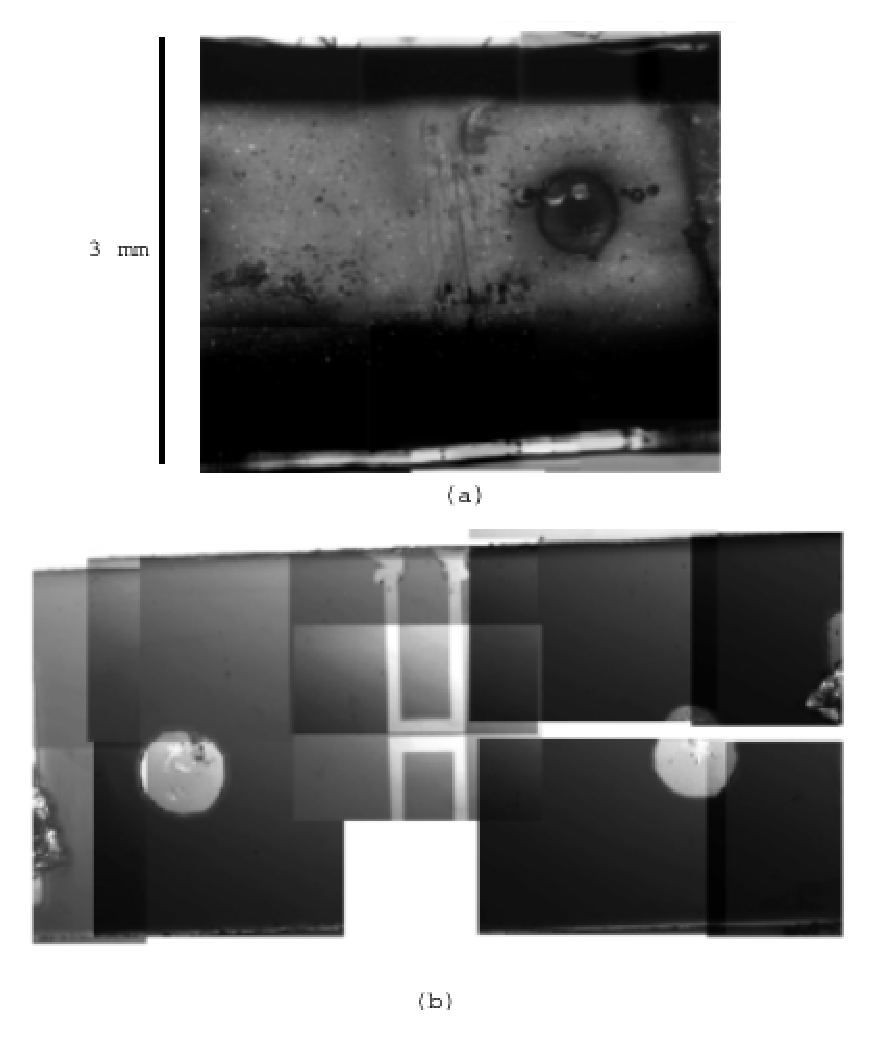
\includegraphics[height=6.0in]{figs/magpen/fig1.ps}
\caption[Optical micrographs of YBCO deposited on RABiTS and STO.]
{(a)Optical micrograph of YBCO deposited on RABiTS. The grains
are observable and are about $50\,\micron$ across. Additionally,
there are small holes evident in the film. These small holes
are approximately $100\,\micron$ apart.
(b) Optical micrograph of YBCO deposited on STO. There are none 
of the pin holes evident in the RABiTS image. This sample has a
microbridge for transport measurements, patterned into the center
via chemical etching. These are montage images, formed from several
different pictures: straight horizontal and vertical lines are
artifacts and not real features of the samples. }
\label{fig:optical_rabits}
\end{figure}

\subsection{Magnetic penetration into YBCO films}

Because RABiTS samples are deposited on nickel, they are 
ferromagnetic from room temperature down to $4.2\,\kelvin$. 
In order to distinguish properties of the YBCO films
from properties of the RABiTS we also looked at magnetic penetration into 
YBCO films 
deposited on STO.
%\footnote{The results of this study of magnetic
%penetration into YBCO films have lead to one publication, 
%Ref.~\cite{nielsen_magpen}.}
An optical image of this sample is shown in \MultFigRef{fig:optical_rabits}{b}.
This particular sample%
\footnote{ORNL sample designation \texttt{la100899}.} 
is YBCO deposited on STO using the same
deposition parameters used in making the YBCO on RABiTS sample 
discussed previously. Additionally, the YBCO/STO sample has been
etched in the center to form a small microbridge in the center. 


%
% Geometry discussion
%
For our discussions, we use the sample geometry defined in 
Fig.~\ref{fig:geometry}, in which we apply the magnetic field
along the $z$ axis, parallel to the thickness $d$ of the film. 
The width of the sample extends from $-W < x < W$ and the length
of the sample extends in the $y$ direction.

%
% fig2 - sample geometry
%
% sample geometry
% this geometry figure was not in the original paper outline,
% but seems useful to describe what's going on. 
%
\begin{figure}[p]
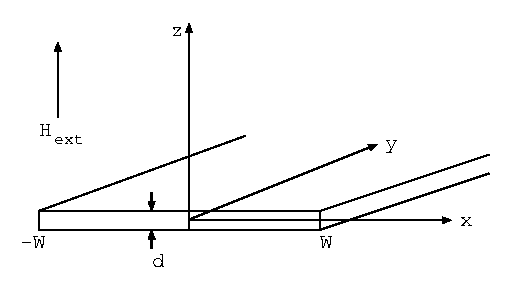
\includegraphics{figs/magpen/fig2.eps}
\caption[Sample geometry used magnetic penetration experiment analysis.]
{Sample geometry used in the experiment and discussion.
The external field is applied along the $z$-axis, through the 
thickness of the film $d$. The sample width extends from $-W < x < W$,
$W=1.5\,\mathrm{mm}$
and we treat the sample as infinitely long in the $y$ direction. 
}
\label{fig:geometry}
\end{figure}


\afterpage{\clearpage}

There has been significant theoretical 
discussion of this problem, in several different limits related
to the film thickness and width. 
In the extreme thin film limit (film 
thickness much less than the penetration depth) Larkin and Ovchinikov
\cite{larkin_jetp_34_651_1972} made the first calculations 
and derived the integral equations necessary to be solved for 
the current distribution in the Meissner state. 
The geometry is as described above, with the sample infinitely
long in the $y$ direction, and a current distribution 
dependent only upon $x$. 
Dorsey \cite{dorsey_prb_51_15329_1995}  took the
integral equations and derived analytic results valid over the 
entire width of the 
superconductor. For thicker films (film thickness comparable
to or larger than the penetration depth) Brandt
\cite{brandt_prl_71_2821_1993,brandt_prb_49_9024_1994,brandt_prb_54_4246_1996}
and Brandt and Mikitik \cite{brandt_prl_85_4164_2000} have made 
considerable numerical progress in describing the current distributions
over the cross-section of a superconducting slab and finally
Vodolazov and Maksimov \cite{vodolazov_physc_349_125_2001} have computed
analytic expressions for the current distributions. Up to now,
there have been no reported measurements of the current distribution
nor magnetic field distribution
in superconducting films
in the Meissner state.

The onset of flux penetration into a superconducting slab has also
been of considerable interest. There exists a large body
of theoretical work, from the geometrical barrier ideas of 
Zeldov \etal\,\cite{zeldov_prl_73_1428_1994} to the edge 
pinning ideas of Kuznetsov \etal\,\cite{kuznetsov_prb_59_1507_1999}
which discuss remanence in a superconducting slab. 
Furthermore, there have been experimental studies of the Bean
critical state in a superconducting slab by Johansen \etal\,
\cite{johansen_prb_54_16264_1996} using magneto optical indicator
\index{magneto optical indicator films}
films (MOIF) and by Ferdeghini \etal\,\cite{ferdeghini_physc_294_233_1998} 
\index{Hall probe}
using a scanning Hall probe. (Because of the large demagnetizing 
factor, initial flux penetration occurs for very low applied fields
and neither of
these techniques are sensitive to fields in this range.)

%
% RABITS
%

\section{YBCO on RABiTS}
\index{RABiTS|(emph}

RABiTS tapes are primarily nickel
\cite{feldman_apl_77_2000,feldman_2000,rabits_web} and it has been
previously reported that they contain a Landau type domain 
structure \cite{landau_physzs_8_153_1935,kercher_prb_60_6878_2000} 
in their 
cross-section. It is now known that this domain structure
cannot exist \cite{arrott_physb_233_259_1997,hertel_prb_60_7366_1999}, 
so we do not expect to find
this type of domain structure. In fact, we do not find any sort of 
simple magnetic domain structure. We imaged a RABiTS substrate%
\footnote{ORNL sample designation \texttt{n020898}.}
without any
superconducting layer deposited, shown in \FigRef{fig:naked_rabits},
and we estimate the height of the SQUID to be between fifty and 
one hundred micrometers for this scan.  
It is clear from the image that the sample is tilted with respect
to the plane of the SQUID.
In the image, the signals
are much clearer and stronger near the right side of the image, but 
fade out near the left edge of the sample. (We know 
the sample is tilted by making contact with the SQUID at 
different points and noting the difference in contact height.)
The magnetic image clearly demonstrates that the spontaneous
magnetization of the RABiTS film is very complicated. 
We did not attempt to demagnetize or magnetize the substrate in any
particular fashion because we wanted to image
the sample as it would (presumably) be if it were used commercially,
as there is no discussion of special magnetic preparation in the 
literature. 

%
% fig3 - naked rabits magnetic picture
%
\begin{figure}[p]
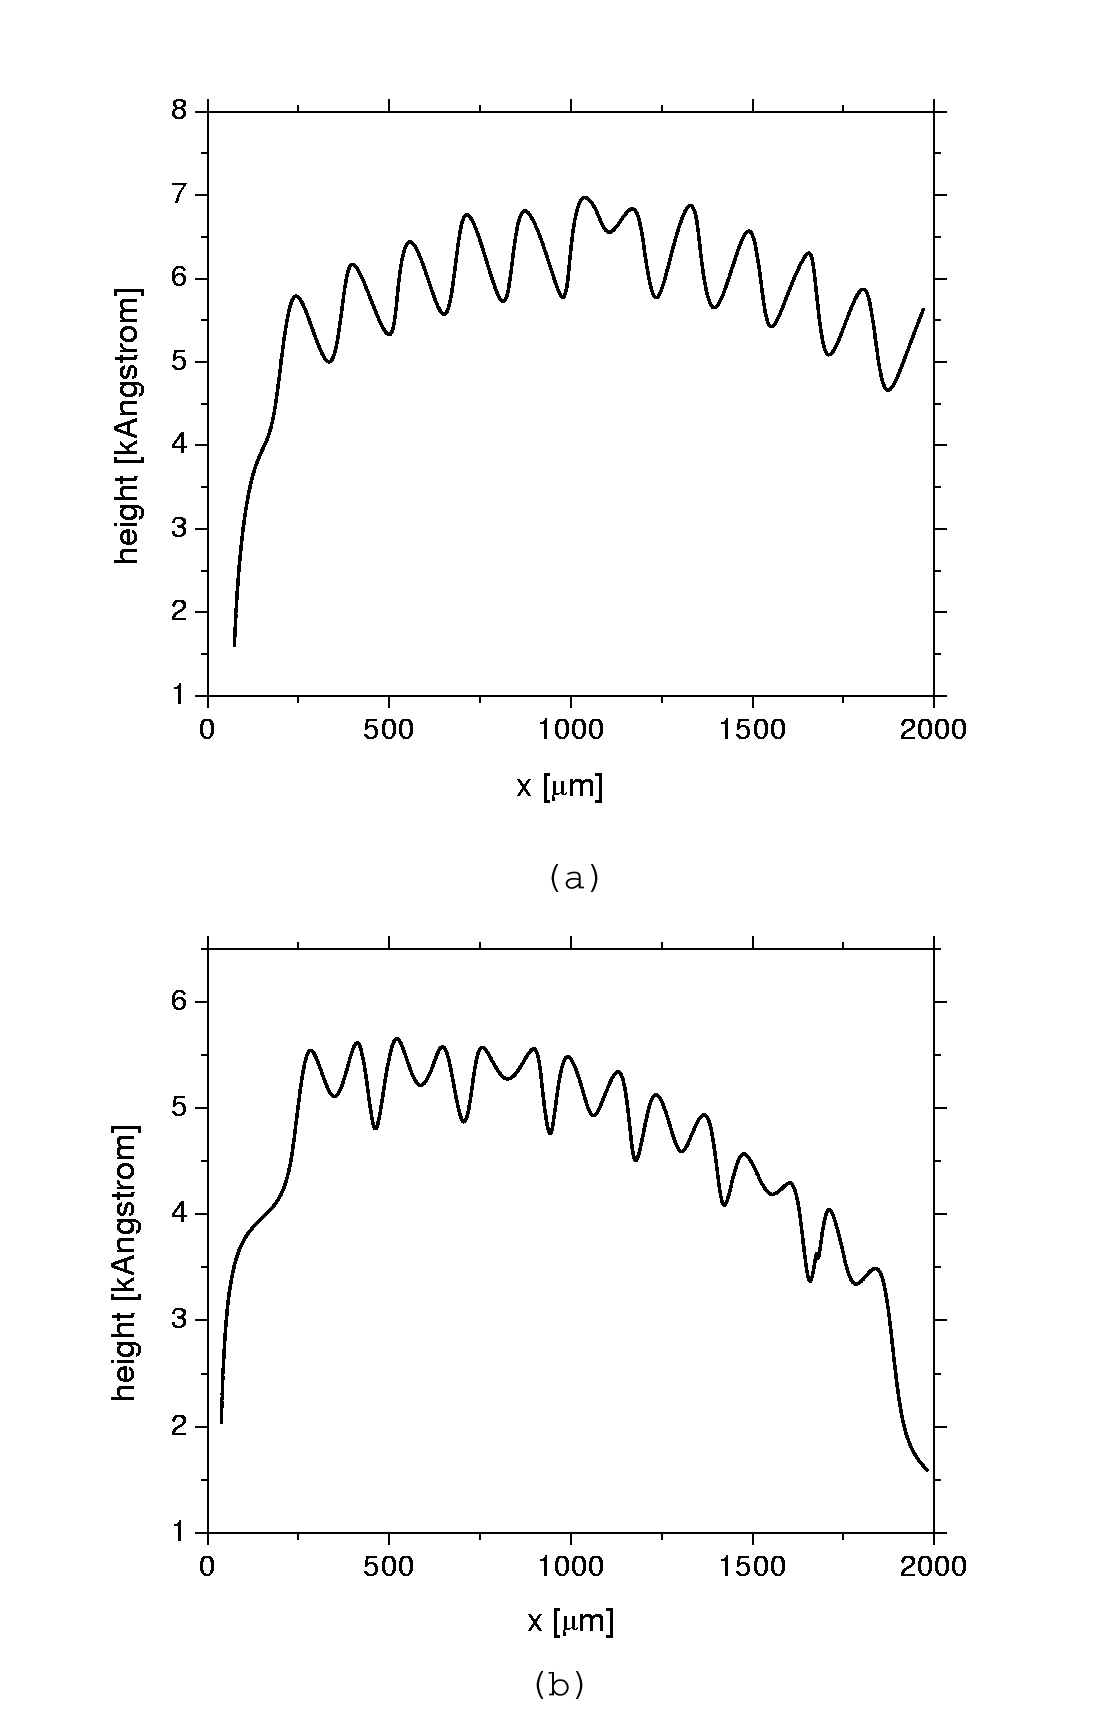
\includegraphics{figs/magpen/fig3.ps}
\caption[Magnetic image of bare RABiTS substrate.]
{Magnetic image of bare RABiTS substrate with spatial units along the
axes shown in millimeters.  The grey scale ranges from
black (low) to white (high) with a difference of  $6.75\,\Gauss$.
The image was taken at $4.2\,\kelvin$. The SQUID height is not 
constant over the surface of the sample; it is closer on the right,
and farther away on the left.}
\label{fig:naked_rabits} 
\end{figure}

Because of these measurements we realized that, using this type of 
substrate, we would be able to cool the sample in zero
\emph{external} field, but that the superconductor would always
see an extremely strong field due to the magnetization of the substrate. 
Hence, the superconductor deposited on RABiTS cannot be cooled in 
zero field.
We demonstrate this by showing, in \FigRef{fig:rabits_zfc},
a nominally zero-field cooled image of YBCO deposited onto RABiTS. 
There have been reports claiming to observe a geometrical barrier
\cite{zeldov_prl_73_1428_1994} in YBCO/RABiTS
\cite{kercher_prb_60_6878_2000}. However, it is not clear that this
should be the case since the YBCO film on RABiTS never sees 
a uniform external field, and further because of the holes in the 
sample we expect flux pinning to be quite strong; the geometrical
barrier requires extremely weak pinning (it was first observed in
single crystals). 

Because of the impossibility of zero field cooling, we
decided to look at YBCO deposited onto STO instead of the 
RABiTS tapes,\footnote{See section~\ref{sec:magpen_ybco},
p.~\pageref{sec:magpen_ybco}.} and investigate the existence of the
geometrical barrier.

\index{RABiTS|)}

%
% fig4 - ZFC YBCO on RABiTS
%
\begin{figure}[p]
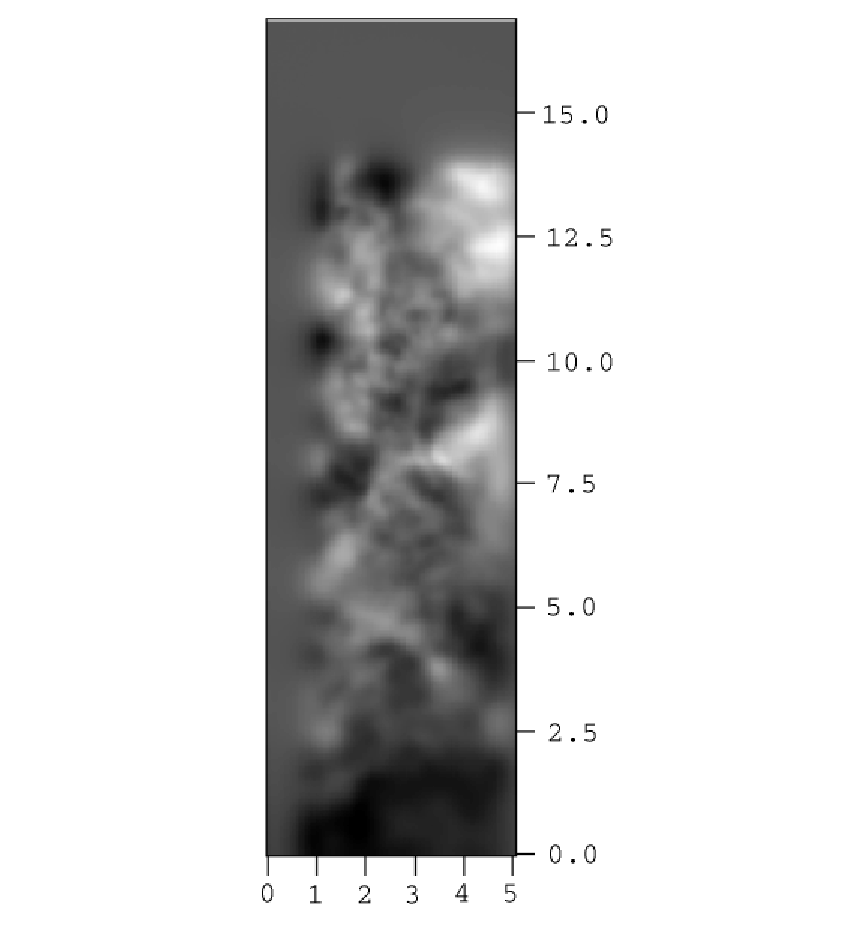
\includegraphics{figs/magpen/fig4.ps}
\caption[Magnetic image of zero field cooled YBCO on RABiTS.]
{Magnetic image of YBCO on RABiTS, cooled in zero external field
to $4.2\,\kelvin$, with the spatial units along the axes shown
in millimeters. 
The grey scale runs from black (low) to white (high) with a 
range of $4.75\,\Gauss$. The plane of the sample is tilted
with respect to the plane of the SQUID, causing the SQUID to 
be closer to the sample in the right of the image. This causes
the image to appear washed out at the left hand side of the image.}
\label{fig:rabits_zfc}
\end{figure}

%
% AC susceptibility measurements. 
%
\subsection{RABiTS AC susceptibility}
\index{AC susceptibility|(emph}
\index{RABiTS!AC susceptibility}
\label{sec:rabits_ac_sus}

In order to understand the basic mechanism involved with loss in
YBCO on RABiTS when carrying current, we used the SQUID to perform a local
measurement of the AC susceptibility at $500\,\Hz$ and 
$1\,\kHz$. 
We use the same experimental arrangement shown in 
\FigRef{fig:pme_experimental_setup}, except that instead of 
applying a DC field with the solenoid, we apply an AC field. 
We use an EG\&G model 5210
lock-in amplifier\cite{EGG} to measure the applied frequency
component in the output from the SQUID electronics. 
From the 
lock-in amplifier we acquire two spatially resolved signals, 
the in phase component and the out of phase component

We can relate these two components to the real and imaginary parts
of the AC susceptibility for the sample. In general the susceptibility is
defined from 
$\vec H = \vec {\vec \chi} \vec M$, in which $\vec{ \vec \chi}$ is the 
susceptibility, a tensor quantity,
$\vec H$ is the magnetic field, $\vec M$ is the magnetization
of the sample. If we assume that material is linear and isotropic, then 
$\chi = H/M$ and for a superconductor in the Meissner state
$\chi=-1$.\footnote{We strive to use MKS units, in which the proper
field relationship for various magnetic quantities is 
$\vec B=\mu_0(\vec H+\vec M)$,
throughout this 
discussion. A very useful chart for conversion between different
electromagnetic unit systems is in Jackson \cite{jackson}, p.~819.}

The sample sees an external driving field of
%
\begin{equation}
H_{\mathrm{ext}}(t) \, \hat z = H_{\mathrm{ac}}\cos(\omega t)\, \hat z
\end{equation}
%
The $\hat z$ component of the sample magnetization 
may be expressed as a series of
Fourier components related to the drive frequency, $\omega/2\pi$,
%
\begin{equation}
M(t) = H_{\mathrm{ac}} \sum_{n=1}^{\infty} 
\left[ \chi_n' \cos (n \omega t) - \chi_n'' \sin (n \omega t) \right]
\end{equation}
in which $\chi_n=\chi_n' + \mi \chi_n''$ is the complex susceptibility
at each frequency component, $n\omega/2\pi$. 
We discuss only the first component, $n=1$,
(hereafter referred to as $\chi$) though 
harmonic generation has been studied in some detail by others 
in bulk measurements
\cite{ishida_prb_41_8937_1990,yamamoto_prb_46_1122_1992}. 

We measure with the lock-in amplifier two components at the driving
frequency, $\omega/2 \pi$, one which is in phase with the driving 
field and one which is $\pi/2$ out of phase with the driving field.
These two components correspond to the real and imaginary 
components of $\chi$. 
The real part, $\chi'$,  corresponds to 
Meissner screening currents within the sample, which are not lossy and 
the imaginary part, $\chi''$, corresponds to processes which cause loss, 
eddy currents in the substrate and hysteretic process in the superconductor
or substrate. 
\index{AC susceptibility|)}

We used a driving amplitude of $223\,\mOe$ for these
measurements. A comparison of the sample response
is shown in \FigRef{fig:rabits_ac_images_a} and 
\FigRef{fig:rabits_ac_images_b} for two excitation
frequencies. 
The signals in these images consist of the YBCO
response and the nickel response. In general the response of both
the media must be considered together in a self-consistent manner, 
but we will discuss the effects separately first and some simplifications
to the self-consistent problem second. 


%
% fig5 part 1 - AC susceptibility images
%
\begin{figure}[p]
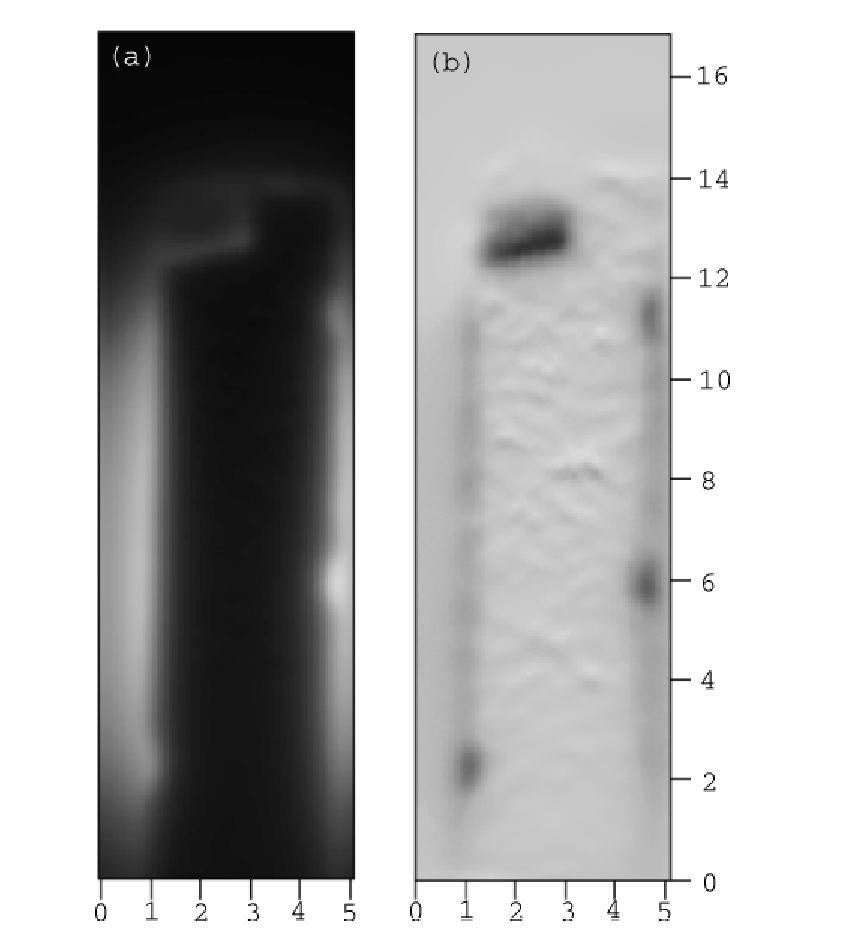
\includegraphics{figs/magpen/fig5r3a.ps}
\caption[YBCO on RABiTS AC susceptibility images at $1\,\kHz$.]
{AC susceptibility images for the YBCO on RABiTS sample, 
zero-field cooled to $4.2\,\kelvin$, 
for an external excitation frequency  
$1\,\kHz$ and
an amplitude of $223\,\mOe$
The spatial dimensions along both 
axes are in millimeters. 
(a) The $\chi'$ image whose grey scale ranges from
$-0.015\,\Gauss$ (black) to $0.25\,\Gauss$ (white).
(b) The $\chi''$ image whose grey scale ranges from  
$-0.045\,\Gauss$ (black) to $0.01\,\Gauss$ (white). 
}
\label{fig:rabits_ac_images_a}
\end{figure}

%
% fig5 part 2 - AC susceptibility images
% 	part 1 and 2 were split into two images to make the images 
%	end up larger when displayed. 
%
\begin{figure}[p]
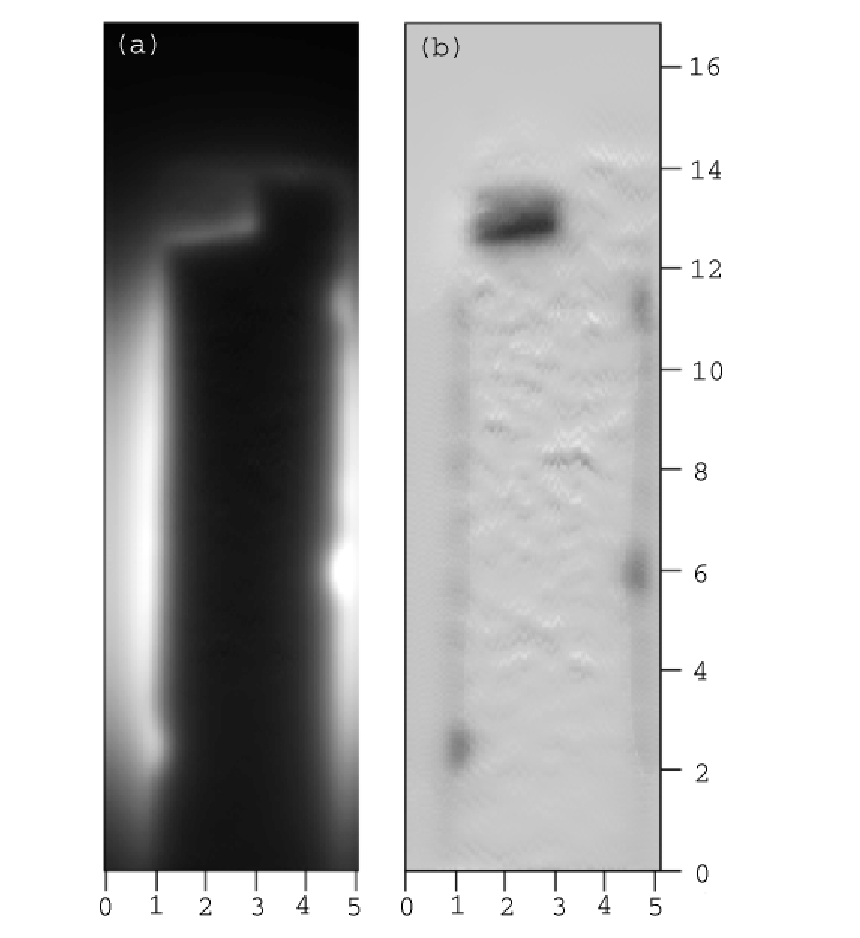
\includegraphics{figs/magpen/fig5r3b.ps}
\caption[YBCO on RABiTS AC susceptibility images at $500\,\kHz$.]
{AC susceptibility images for the YBCO on RABiTS sample, 
zero-field cooled to $4.2\,\kelvin$ for an external excitation frequency  
$500\,\Hz$ and
an amplitude of $223\,\mOe$. The spatial dimensions along both 
axes are in millimeters. 
(a) The $\chi'$ image whose grey scale ranges from
$-0.015\,\Gauss$ (black) to $0.25\,\Gauss$ (white).
(b)  The $\chi''$ image, whose grey scale ranges from
$-0.045\,\Gauss$ (black) to $0.01\,\Gauss$ (white). 
}
\label{fig:rabits_ac_images_b}
\end{figure}

We can understand the eddy current generation in the substrate by 
considering Maxwell's equations and Ohm's Law. 
We start by taking the curl of
Ohm's Law which gives
%
\begin{equation}
\nabla \times \vec{J}(\vec{x},t) = \sigma \nabla \times \vec{E}(\vec{x},t) 
= -\sigma 
{\dif  \over \dif t} \vec{B}(\vec{x},t) \mbox{.}
\label{eqn:eddy_curr_deriv}
\end{equation}
%
Additionally, we assume that the material response is linear 
so that
$\vec{B}(\vec{x},t) = \vec{B}(\vec{x})\me^{\mi \omega t}$
and $\vec{J}(\vec{x},t) = \vec{J}(\vec{x})\me^{\mi \omega t}$
which we substitute into \EqnRef{eqn:eddy_curr_deriv} to get
%
\index{eddy currents}
\begin{equation}
- \nabla \times \delta^2 \vec{J}(\vec{x}) = {\mi \over \mu_0} \vec{B}(\vec{x})
\label{eqn:eddy_current_screening}
\end{equation}
%
in which $\delta=\sqrt{1/\mu_0\sigma \omega}$ is the skin depth,%
\footnote{This skin depth differs from the skin depth as conventionally
defined by a factor of $\sqrt{2}$, see Jackson\cite{jackson}, p.~298 or 
Panofsky and Phillips\cite{panofsky_phillips}.}
$\mu_0$ is the permeability of free space, 
$\sigma$ is the 
conductivity of the material, $\omega/2\pi$ is the driving 
frequency, $\vec{J}(\vec{x})$ is the
induced eddy current and $\vec{B}(\vec{x})$ is the total magnetic induction. 
It's clear that the eddy current is out of phase with the 
drive field by a phase of $\pi/2$, which is why we expect the
field generated by the eddy currents to affect the $\chi''$ signal. 

It's interesting to note the similarity between 
\EqnRef{eqn:eddy_current_screening}\ and the London equation
(in MKS units)%
\footnote{See Tinkham\cite{tinkham}, p.~4 for the London equations.
We have neglected the time dependence 
of $\vec{J}$ and $\vec{B}$. In general these are time dependent 
quantities, but here we consider the DC Meissner response.}
%
\index{London equation}
\begin{equation}
- \nabla \times \lambda^2 \vec{J}(\vec{x}) = \vec{B}(\vec{x})
\label{eqn:London_equation}
\end{equation}
%
\index{London penetration depth}%
\index{$\lambda$|see{London penetration depth}}%
in which $\lambda$ is the London penetration depth, $\vec{J}(\vec{x})$ is the 
Meissner current and $\vec{B}(\vec{x})$ 
is the total magnetic induction. In our 
geometry, the shape of the current distribution $\vec{J}(\vec{x})$ will be 
the same for both \EqnRef{eqn:eddy_current_screening} and 
\EqnRef{eqn:London_equation}. The primary difference is that
the eddy current screening is out of phase with the drive field,
while Meissner current screening is in phase with the drive field
(and the Meissner current may flow at DC). 

As discussed above, we expect to see the eddy current response of the nickel
in the $\chi''$ image. However, the nickel is below (and hence
screened) by the YBCO, so we do not necessarily expect the 
nickel to actually see the driving field and respond,
except in regions where the YBCO fails to screen. 
In fact this is exactly what we see. 
In \MultFigRef{fig:rabits_ac_images_a}{a}, which shows
$\chi'$,
there is a light 
region in the upper right corner of the sample which does
not screen the external field. Darker colors are screening
regions in this case because they are closer to zero field.
This same region in 
\MultFigRef{fig:rabits_ac_images_a}{b}, $\chi''$, 
shows the strongest response 
indicating that the YBCO is not superconducting in 
this region and hence not screening the nickel tape underneath. 
In addition to this region, there are other regions which have the 
same correlation between the two images, particularly at the edges of 
the sample.

We can understand these measurements more quantitatively by 
considering separately the AC response of the YBCO and the nickel
substrate. At our low temperature ($4.2\,\kelvin$) and field amplitude
(below $H_{c1f}$),
we expect the sample to be in the Meissner state, and so we expect to
observe Meissner shielding in phase with the driving field. 
We could not cool the sample in zero field due to the presence of the 
substrate. The substrate provides a DC magnetic field, if the pinning
in the sample is strong enough, this DC field will be pinned and
when we measure AC excitations of the sample, we expect to find
a Meissner screening response at the same frequency as the driving 
field.
Line cuts through the $\chi'$ magnetic images in 
\FigRef{fig:rabits_ac_images_a} and 
\FigRef{fig:rabits_ac_images_b}\ at $x=9.1\,\mm$ are shown in 
\FigRef{fig:rabits_ac_line_cuts_a}, and qualitatively show the expected
Meissner screening form.\footnote{We discuss Meissner screening
in great detail in section \ref{sec:ybco_meissner_state}, 
p.~\pageref{sec:ybco_meissner_state}. We note here that these
AC susceptibility measurements agree with the Meissner state
discussion below.} 

%By considering the images, several features become immediately
%obvious. We can see that there appears to be some form of damage to 
%the sample, degrading the superconductivity in the sample when
%we compare \FigRef{fig:rabits_ac_images}. Consider the dark
%regions in \FigRef{fig:rabits_ac_images}(b) and (d) which indicate
%that the sample is lossy. These regions correspond to regions in 
%\FigRef{fig:rabits_ac_images}(a) and (c)  in which there 
%is no screening response. All of these regions occur near the 
%edge of the sample, indicating that there has been some 
%damage to the sample near the edges, causing the loss of 
%superconductivity in those regions. It is likely that these lossy 
%regions are actually the nickel eddy current response, as
%discussed above. 

%
% recombine these into one figure
%
\begin{figure}[p]
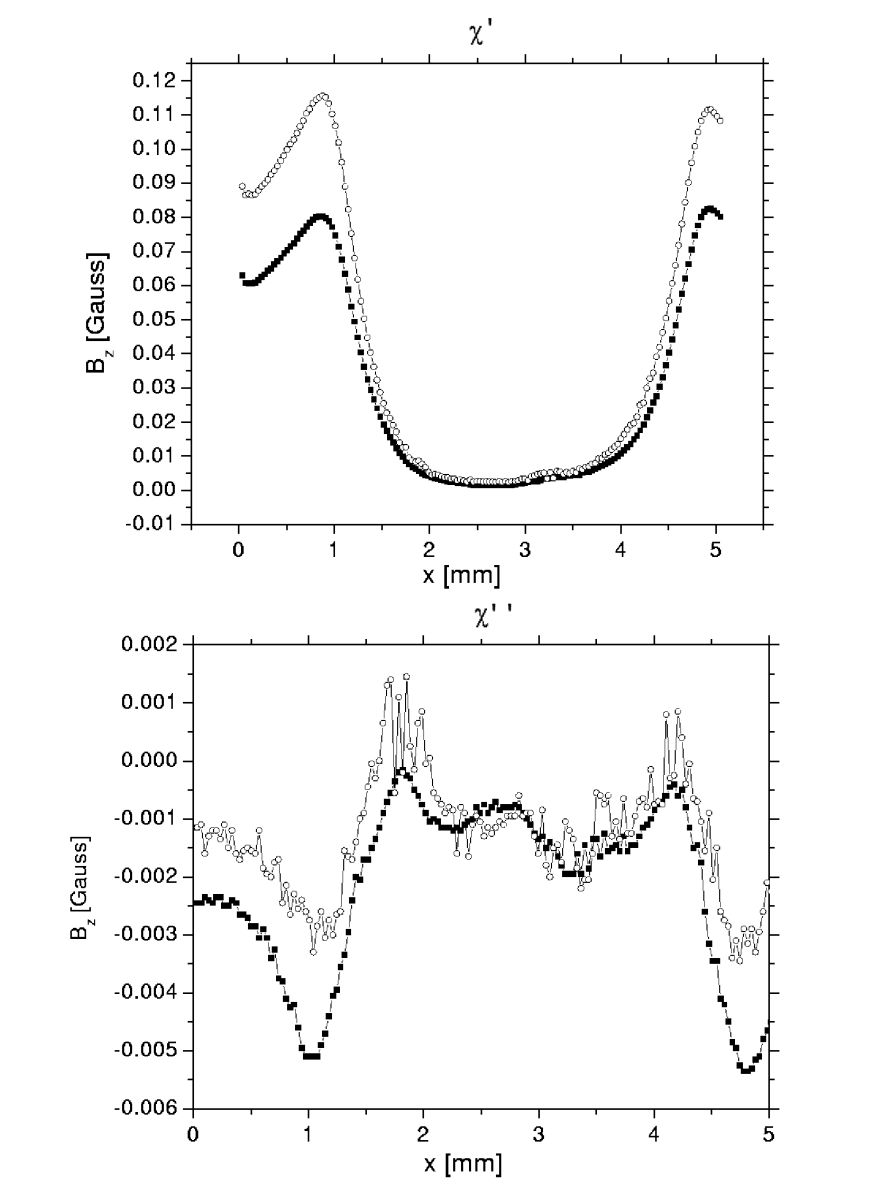
\includegraphics[width=5.7in]{figs/magpen/ac.ps}
\caption[$\chi'$ and $\chi''$ line cuts through AC 
susceptibility measurements.]
{$\chi'$  and $\chi''$ 
line cuts through AC susceptibility measurements taken at 
$x=9.1\,\mm$, for $1\,\kHz$ (black squares) and
$500\,\Hz$ (open circles).
}
\label{fig:rabits_ac_line_cuts_a}
\label{fig:rabits_ac_line_cuts_b}
\end{figure}

%  part 1
% line cuts through ac sus images
%
%\begin{figure}
%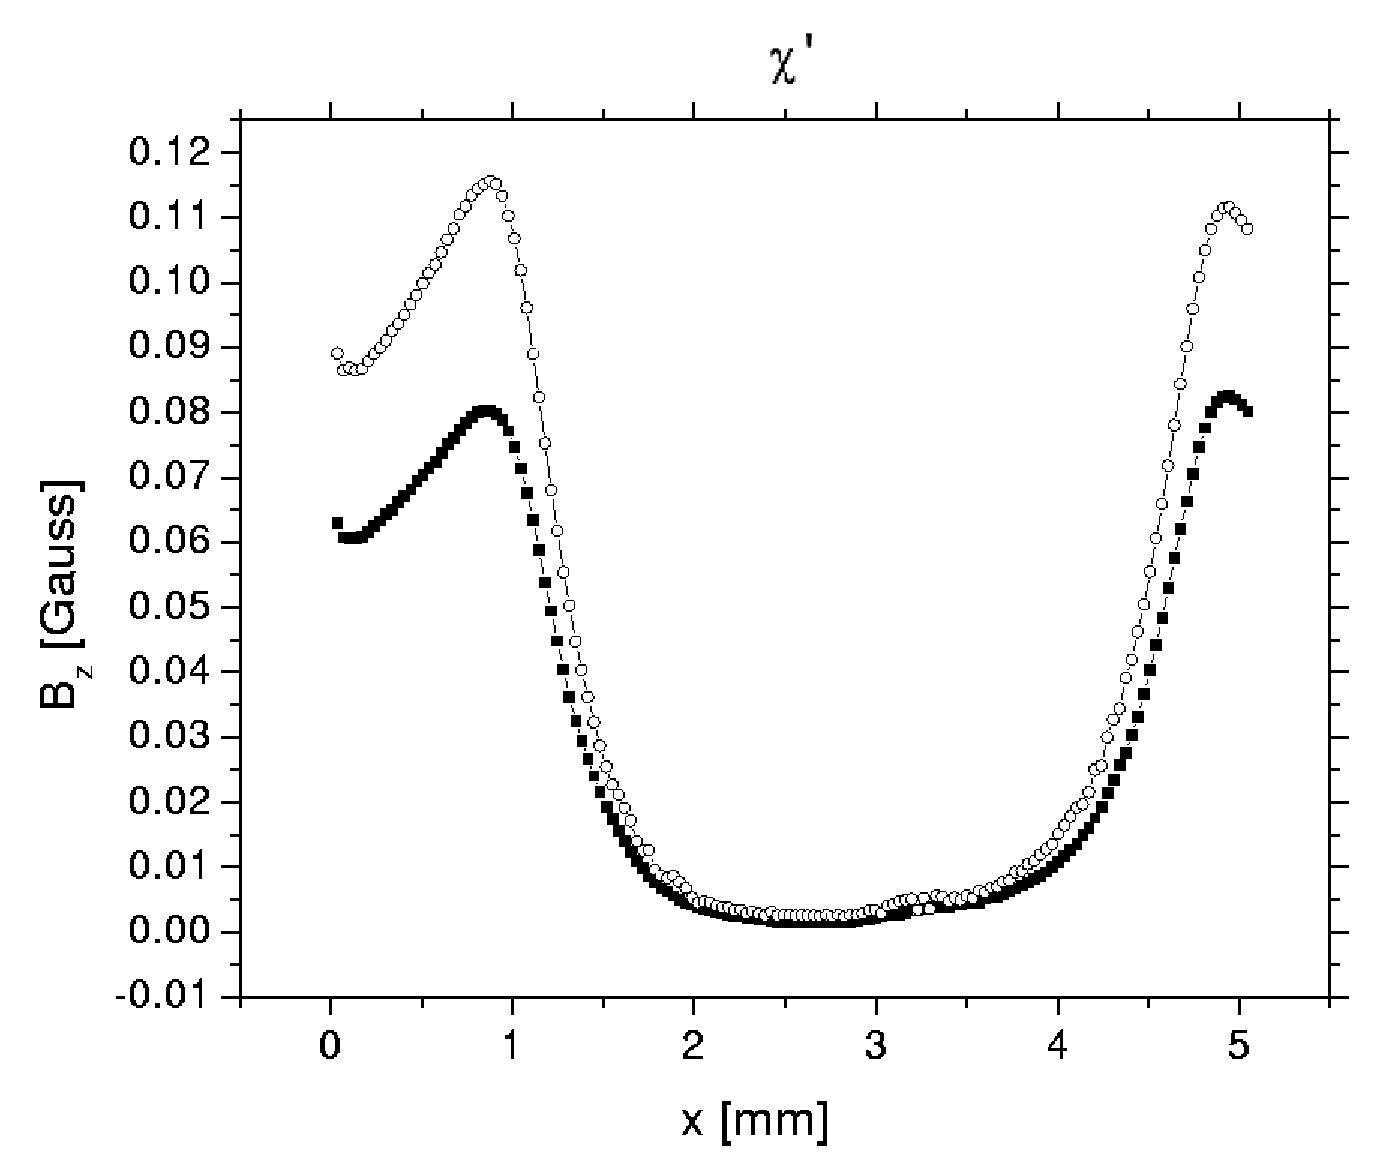
\includegraphics[width=5.7in]{figs/magpen/acinphase.ps}
%\caption[$\chi'$ line cuts through AC susceptibility measurements]
%{$\chi'$ line cuts through AC susceptibility measurements taken at 
%$x=9.1\,\mm$, for $1\,\kHz$ (black squares) and
%$500\,\Hz$ (open circles).
%}
%\label{fig:rabits_ac_line_cuts_a}
%\end{figure}

%  part 2
% line cuts through ac sus images
%
%\begin{figure}
%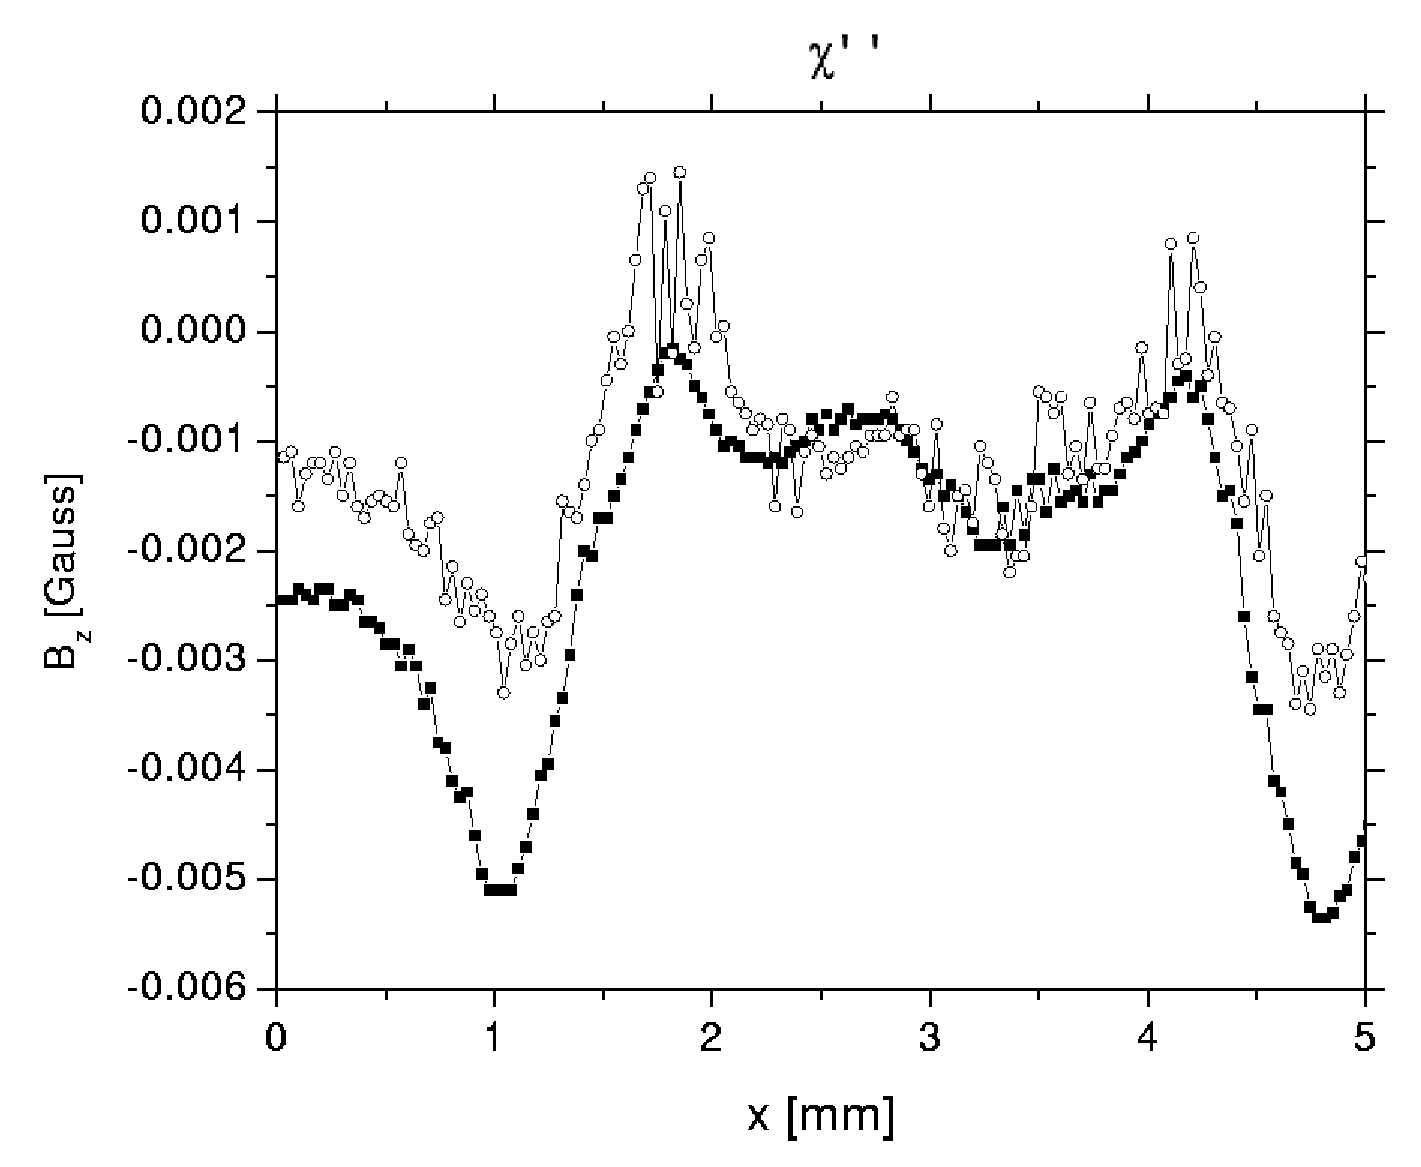
\includegraphics[width=5.7in]{figs/magpen/acoutofphase.ps}
%\caption[$\chi''$ line cuts through AC susceptibility measurements]
%{$\chi''$ line cuts through AC susceptibility measurements taken at 
%$x=9.1\,\mm$, for $1\,\kHz$ (black squares) and
%$500\,\Hz$ (open circles).}
%\label{fig:rabits_ac_line_cuts_b}
%\end{figure}

\label{sec:flux_motion_losses}
In the superconductor itself, we expect to observe losses associated
with motion of flux
for any, arbitrarily low, excitation
field because the spontaneous magnetization of the nickel assures
that flux will always be present in the superconductor. 
Losses due to vortex motion in a superconductor may result 
from different processes, flux-flow resistance
\cite{nikolo_prb_39_6615_1989,clem_mag_sus_1991} and
intergranular (or grain boundary) vortex motion
\cite{celebi_physc_309_131_1998,muller_prb_43_7976_1991}.
It is well known that flux-flow resistance is strongly dependent
upon driving frequency.\footnote{An analogy can be drawn between 
flux-flow resistance and eddy current generation in normal metals,
which as discussed previously, is proportional to the driving 
frequency. See Clem \cite{clem_mag_sus_1991} for an excellent 
description and derivation of the analogy.} 
Moreover, it has been reported that losses due to intergranular 
vortex motion are typically frequency 
independent \cite{celebi_physc_309_131_1998}.

We pointed out previously that because of the large spontaneous
magnetization of the nickel that we could not 
cool the sample in total zero field,
so
we do not expect the sample to be in the Meissner state.
Instead we expect the sample 
to have a complicated internal magnetic structure, which
will respond hysteretically to the excitation field. Hysteretic losses
appear in the out of phase image and provide a means to identify
lossy regions of the sample. Furthermore, by studying the amplitude
and frequency dependence we may determine the cause of the losses in
different regions. There are regions near
the edges of the sample which have strong loss signals, and no Meissner
screening signal. These regions are likely defective YBCO film
and the strong loss signal results from the eddy currents in the nickel. 

It is difficult to do a systematic study of the sample over a wide
frequency and amplitude range because of the time required to generate
the different images. None the less, we have made several images
at a fixed external amplitude, over a range of frequencies from
$500\,\Hz$ to $5\,\kHz$. A selection of these images is shown in 
\FigRef{fig:rabits_ac_images_a}\ and 
\FigRef{fig:rabits_ac_images_b}, with line cuts through these images at
$x=9.1\,\mm$ shown in \FigRef{fig:rabits_ac_line_cuts_a}
and \FigRef{fig:rabits_ac_line_cuts_b}. From the line
cuts in \FigRef{fig:rabits_ac_line_cuts_b} ($\chi''$ or loss images)
we notice that there is considerable internal structure and that 
both line cuts at $500\,\Hz$ and $1\,\kHz$ are remarkably similar. 
Furthermore, we notice that the line cuts do not go to zero outside of the
sample as they should. This indicates that the phase separation between
the in and out of phase signals was incomplete at the lock-in amplifier.
None the less, the loss signal is qualitatively 
frequency independent, indicating that
the losses are occurring at the grain boundaries, rather than in the grains. 

With losses occurring in the grain boundaries, rather than in the 
grains themselves (as flux-flow resistance) we expect that the current
carrying capacity of the YBCO on RABiTS films may be increased by increasing
the size of the grains in the sample. At some point however, the spontaneous
magnetization of the RABiTS substrate will become the limiting factor
for the losses, inducing flux in the YBCO causing flux-flow losses. 
These flux-flow losses would continue to occur even if one could 
engineer a way to deposit a single crystal on the RABiTS. 


%
% DC hysteresis measurements 
%
\subsection{RABiTS DC hysteresis measurements}
\label{sec:rabits_dc_hyst}
\index{DC susceptibility}
\index{RABiTS!DC susceptibility}

In addition to the AC susceptibility measurements we made DC 
hysteresis measurements on the sample in order to investigate
how flux became pinned in the sample. We did this measurement
at two different heights above the sample, approximately $50\,\micron$
and $20\,\micron$, but could only take single line scans at the
closer height because of a tilt in the mounted sample relative
to the scanning plane. 

To generate a hysteresis measurement we take one scan after
zero field cooling; ramp the external field up to a specific
value; ramp the field back to zero; and finally reimage the sample. 
We compare the two images by subtracting the first from the 
second. The resulting difference image should reveal where flux
trapping is hysteric for the particular field.

We show, in \FigRef{fig:dc_hyst_gen_a}(a)-(b) the images before
and after application of the external field and in 
\FigRef{fig:dc_hyst_gen_b}(a) the difference between 
\FigRef{fig:dc_hyst_gen_a}(a)-(b).
The SQUID at a height
between $100\,\micron$ (however, the sample is tilted, as discussed 
above for the bare RABiTS substrate) and  
$50\,\micron$ and a peak applied external field of $223\,\mOe$. 
In addition to the difference image, we compare the 
magnitude of the gradient of the field in 
\MultFigRef{fig:dc_hyst_gen_a}{a}\ $\left| \nabla_{x,y} B_z \right|$
(shown in \MultFigRef{fig:dc_hyst_gen_b}{b}) with the difference 
image in order to verify that the features observed in the 
difference image are not a result of mechanical misalignment
between the two images resulting in a false image.
We do this because two images, exactly the same, but offset slighly
will produce a difference image which contains the strongest
signal near where the gradient of the first two images is largest.
 It is clear 
from comparing \FigRef{fig:dc_hyst_gen_b} (a) and (b) that 
there is some correlation between the two images, indicating that some
of the structure is due to misalignment in the probe mechanics. 

%
% fig6 part 1 - DC hysteresis images
%	these figure numbers no longer refer to numbers in the 
%	text, but they do refer to figures as numbered in the
%	figure directory
%
\begin{figure}[p]
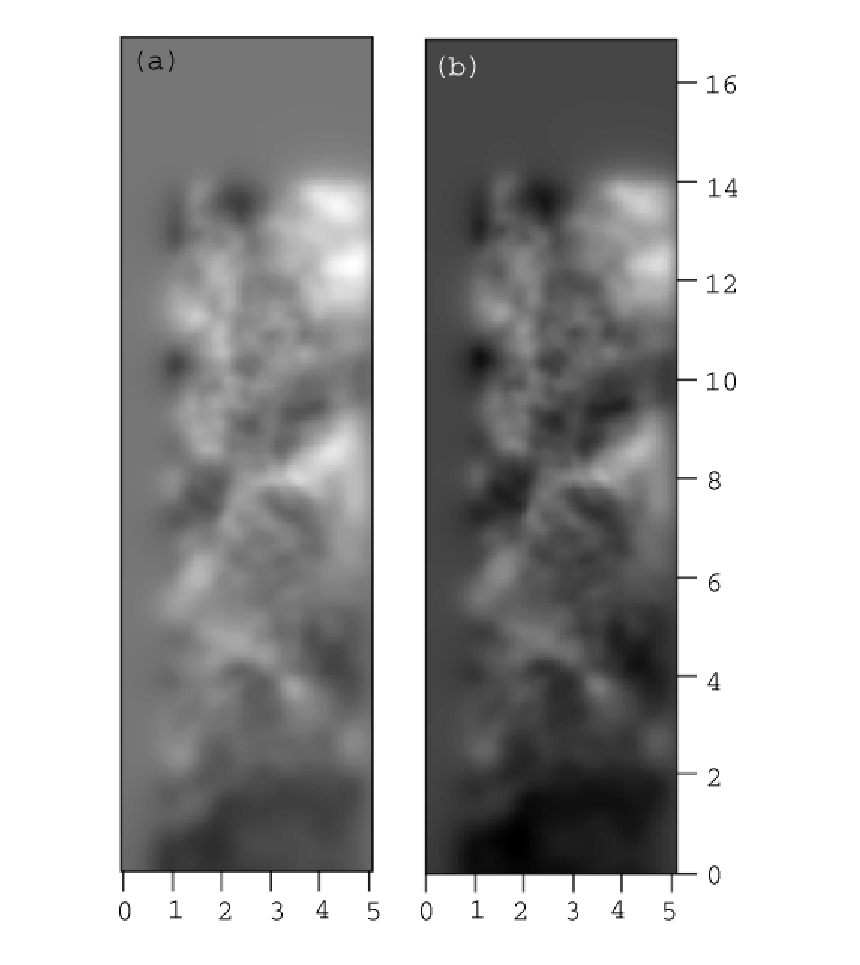
\includegraphics{figs/magpen/fig6a.ps}
\caption[DC hysteresis before and after images of YBCO/RABiTS.]
{Typical images used to study DC hysteresis in the YBCO/RABiTS data
at a height of $50\,\micron$.
(a) Image taken after zero field cooling the sample. The grey
scale ranges from low (black) to high (white) with a total
range of $5.6\,\Gauss$. 
(b) Image taken after ramping the external field to $1.16\,\Gauss$
and subsequently removing the external field before measuring. 
The grey scale is the same as (a). 
}
\label{fig:dc_hyst_gen_a}
\end{figure}

%
% fig6 part 2 - DC hysteresis images
% 	these were split into two parts to make them appear large
% 	in the text
\begin{figure}[p]
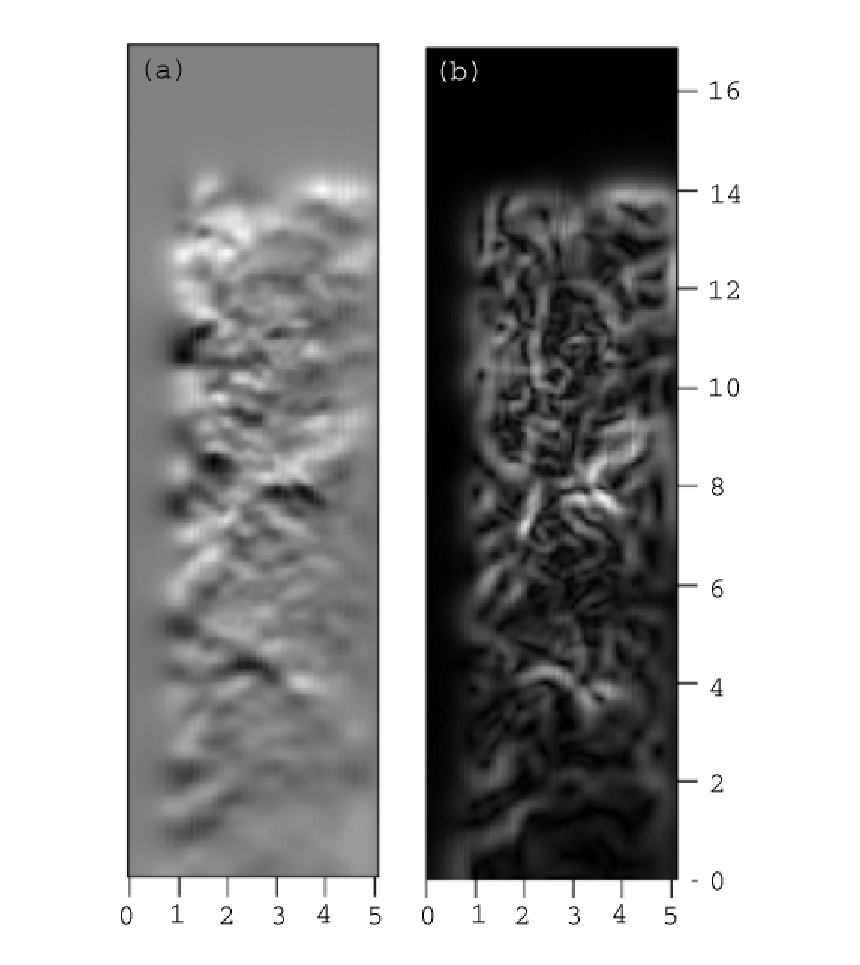
\includegraphics{figs/magpen/fig6b.ps}
\caption[DC hysteresis difference and gradient images of YBCO/RABiTS.]
{Typical images used to study DC hysteresis in the YBCO/RABiTS data
at a height of $50\,\micron$.
(a) Difference image taken by subtracting 
\FigRef{fig:dc_hyst_gen_a}(a) from (b), the grey
scale ranges from $-1.7\,\Gauss$ (black) to $-0.35\,\Gauss$ (white). 
(b) Magnitude of the gradient of the image in (a) for comparison 
with the difference image. The grey scale runs from zero (black) to
$7.3\,\Gauss/\mm$ (white).
}
\label{fig:dc_hyst_gen_b}
\end{figure}

A simple method to correct for this would be to shift one of the 
images in $x$ and $y$ before taking the difference, however
to simplify this comparison process, we took single vertical line scans over 
the sample at a horizontal point of $7.5\,\mm$ in \FigRef{fig:dc_hyst_gen_a}.
These single line scans were taken separately from the images discussed
above and were arranged so that the sample only moved along the single 
line during the data collection. In this way the line scans lie atop
each other and would only need to be shifted in one direction. 
These line scans, shifted to match the peaks 
are shown in \FigRef{fig:dc_hist_cuts_high_a}, 
for both the zero field cooled and hysteresis scans. 
It was not possible to match all of the peaks simultaneously. 
Vertical, numbered lines are drawn in \FigRef{fig:dc_hist_cuts_high_a}
at the location of several peaks. In order to correlate these two
line scans we shifted the curves such that peak 1 occurred at the same
$x$ value for each. After we did this, the location of peak 2 and 4
did not coincide, however the location of peak 3 did. The difference
in the peak coincidence,less than $10\,\micron$,  indicates that either 
the mechanical deviations are not linear across the scan or that
small flux has shifted within the sample on very small length scales. 
The difference 
between these two scan lines is shown in \FigRef{fig:dc_hist_cuts_high_b}
along with the gradient of the zero field cooled line scan for 
comparison. Both line scans are very similar, except for a 
small offset which may be due to a flux jump in the SQUID washer
between line scans.
Furthermore, the gradient of the line scans correlates quite
well with the difference between the two line scans, 
indicating that the difference we are 
measuring is a result of mechanical misalignment in the scanning 
mechanism, rather than real hysteresis. 

\begin{figure}[p]
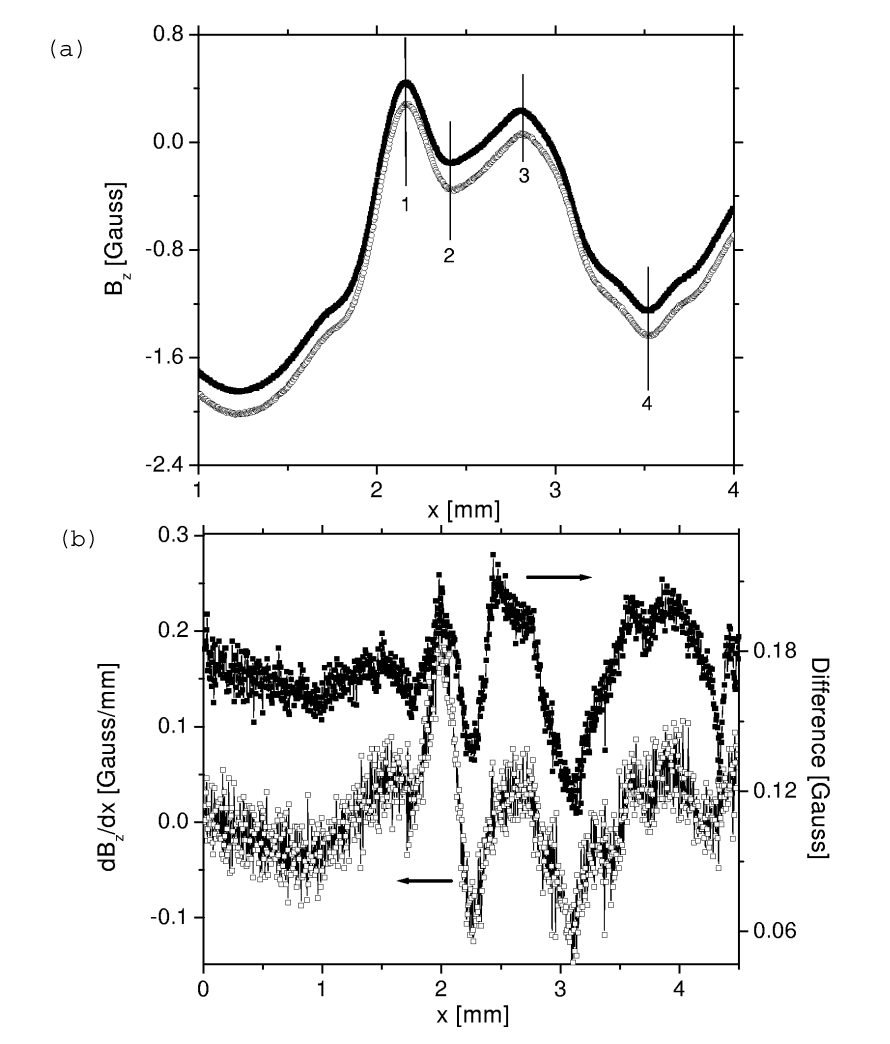
\includegraphics[width=5.7in]{figs/magpen/dcline.ps}
\caption[Before and after line cuts of DC hysteresis 
images at a height of $50\,\micron$.]
{(a) 
Vertical line cuts of DC hysteresis images, with the SQUID at a height of
$50\,\micron$, at $x=7.5\,\mm$. 
Zero field cooled line scan (open circles) and line scan after 
ramping the external field to $1.16\,\Oe$ and back to zero
(black squares). 
(b) Difference (black squares) and gradient (open squares) of the
vertical line cuts.
}
\label{fig:dc_hist_cuts_high_a}
\label{fig:dc_hist_cuts_high_b}
\end{figure}

%
% fig7 - line cuts of DC hysteresis images @ 50 microns
% part 1 - before and after line cuts
%
%\begin{figure}
%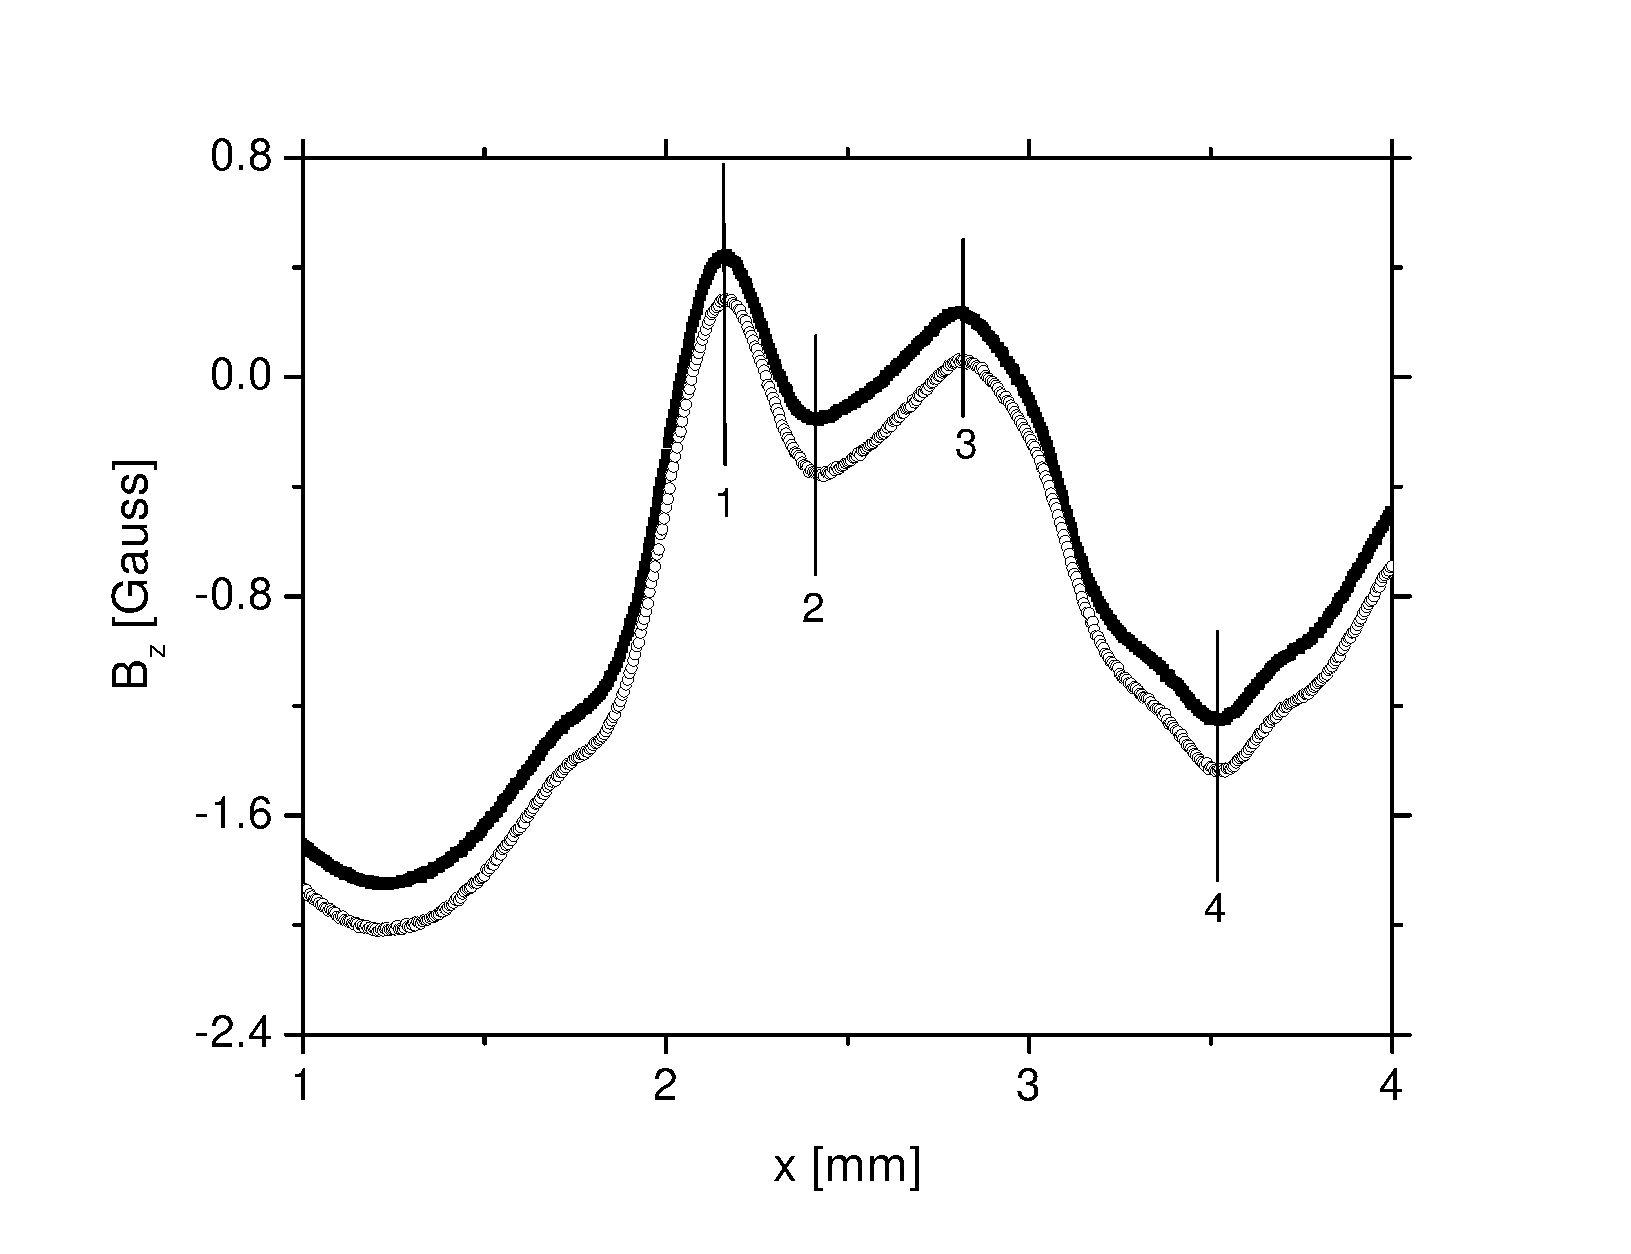
\includegraphics[width=5.7in]{figs/magpen/fig7a.eps}
%\caption[Before and after line cuts of DC hysteresis 
%images at a height of $50\,\micron$.]
%{Vertical line cuts of DC hysteresis images, with the SQUID at a height of
%$50\,\micron$, at $x=7.5\,\mm$. 
%Zero field cooled line scan (open circles) and line scan after 
%ramping the external field to $1.16\,\Oe$ and back to zero
%(black squares). 
%}
%\label{fig:dc_hist_cuts_high_a}
%\end{figure}

%
% fig7 - line cuts of DC hysteresis images @ 50 microns
% part 2  - difference and gradient line cuts
%
%\begin{figure}
%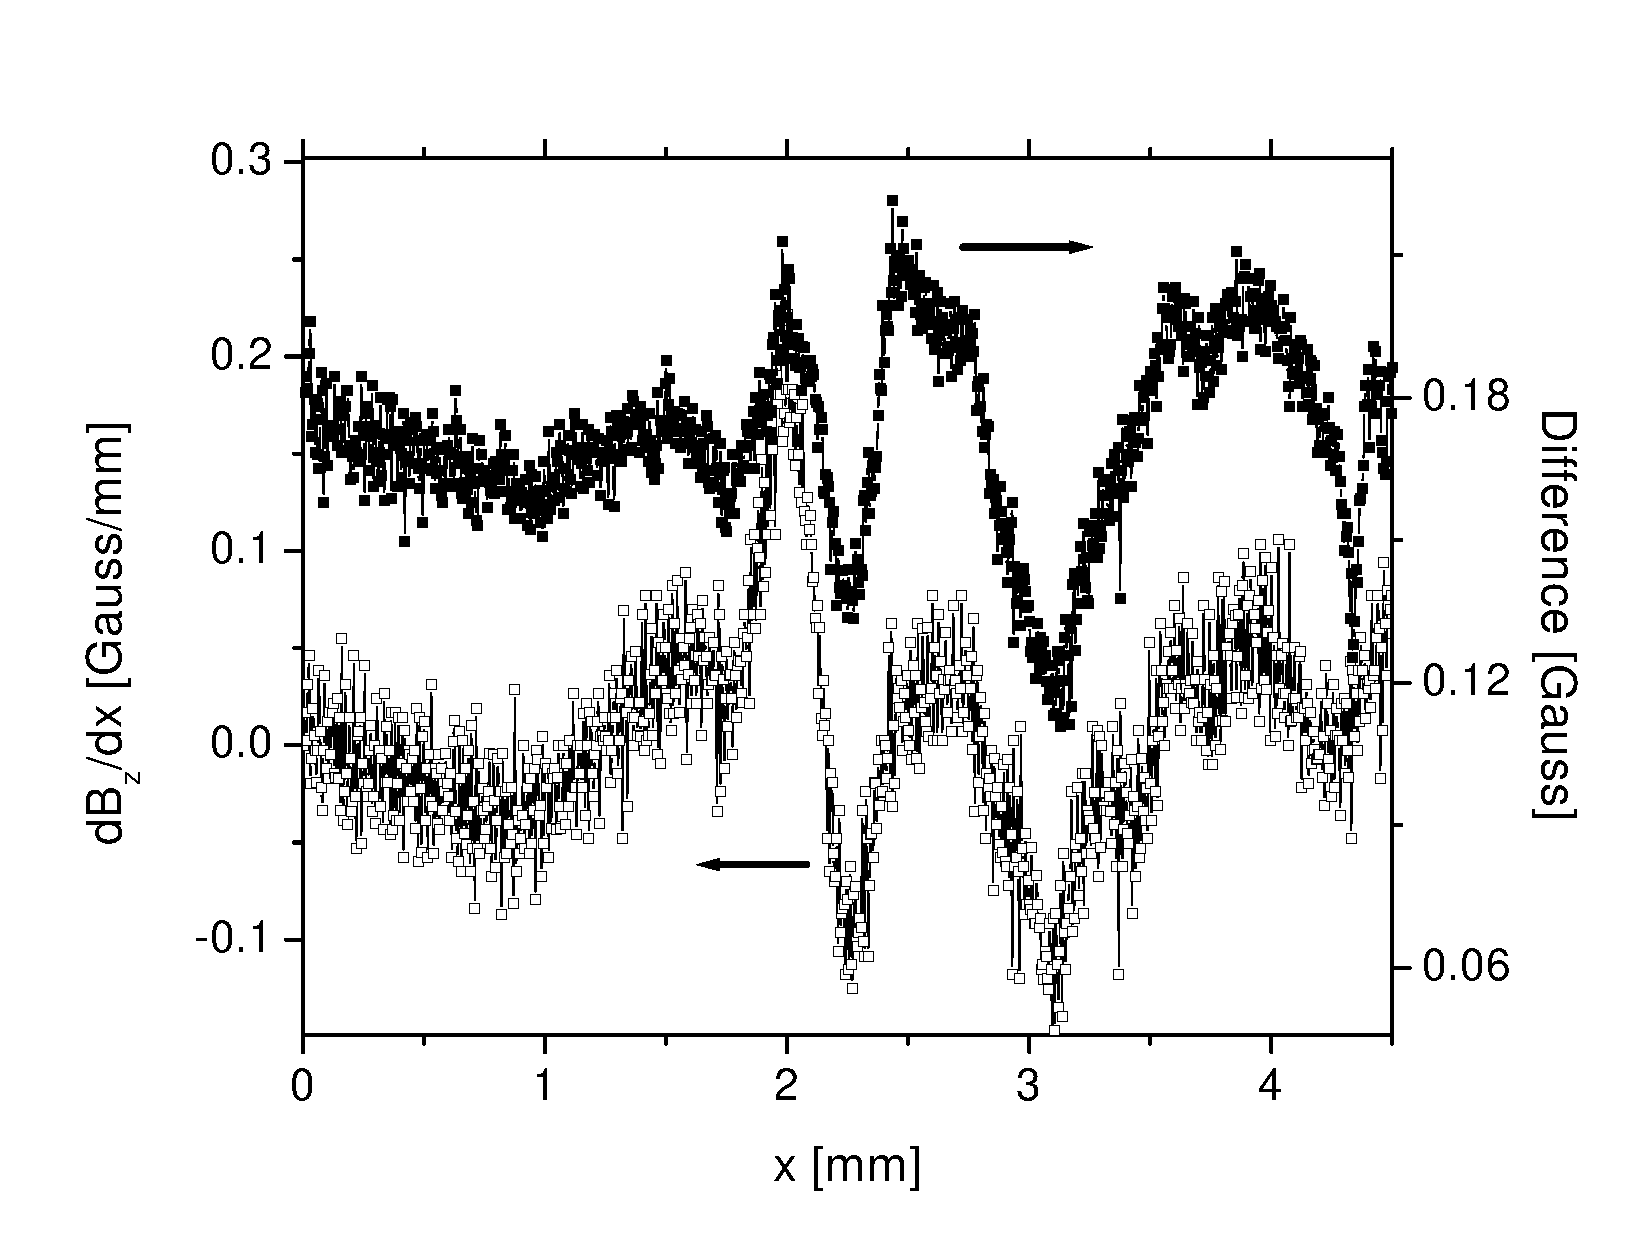
\includegraphics[width=5.7in]{figs/magpen/fig7b.eps}
%\caption[Difference and gradient line cuts of DC hysteresis 
%images at a height of $50\,\micron$.]
%{Vertical line cuts of DC hysteresis images, with the SQUID at a height of
%$50\,\micron$, at $x=7.5\,\mm$. 
%Difference of the two curves in \FigRef{fig:dc_hist_cuts_high_a} 
%(open squares) 
%and the derivative plot 
%of the zero field cooled line scan (black squares).  
%}
%\label{fig:dc_hist_cuts_high_b}
%\end{figure}

In order to improve upon the line scans taken above, we made 
line scans at 
a SQUID height of about $20\,\micron$.
By using these line scans analogously to the line scans 
taken at $50\,\micron$ (\cf\ \FigRef{fig:dc_hist_cuts_high_a}\ )
we were able to observe new features in the sample that were
invisible at the greater height. These line scans are shown in
\FigRef{fig:dc_hist_cuts_low_a} for the same parameters as the
previously discussed line scans. 

Again, the same analysis was performed, comparing the zero
field cooled line scan to a line scan taken after increasing the
external field to $1.16\,\Gauss$ and back to zero. 
Again, for the best 
comparison of the two, we shifted the zero field cooled image left
and right until the peaks matched as closely as possible to the 
line scan taken after applying the external field. 
This helps to eliminate potential errors 
introduced into the difference image because of the gradient of the
magnetic field. The gradient and the difference are shown in 
\FigRef{fig:dc_hist_cuts_low_b} for comparison. The correlation between
the two is not nearly as strong as in the previous case. 

As a better method of comparison, we compare specific locations in 
\FigRef{fig:dc_hist_cuts_low_a}.  
First consider the peaks that are quite evident in both line scans
in \FigRef{fig:dc_hist_cuts_low_a}\ and note that the peaks
are typically separated by about $100\,\micron$, which is the same 
average separation
between the holes in the YBCO as seen in \MultFigRef{fig:optical_rabits}{a}. 
We infer from this that the holes in the YBCO film are harboring 
pinned flux. 
Now compare the 
specific locations in the image indicated 
by arrows which  indicate locations where the height of the 
peaks has changed between line scans.
This change in the height indicates that the amount of flux
pinned in that region has changed during the application
of the external field. 

\begin{figure}[p]
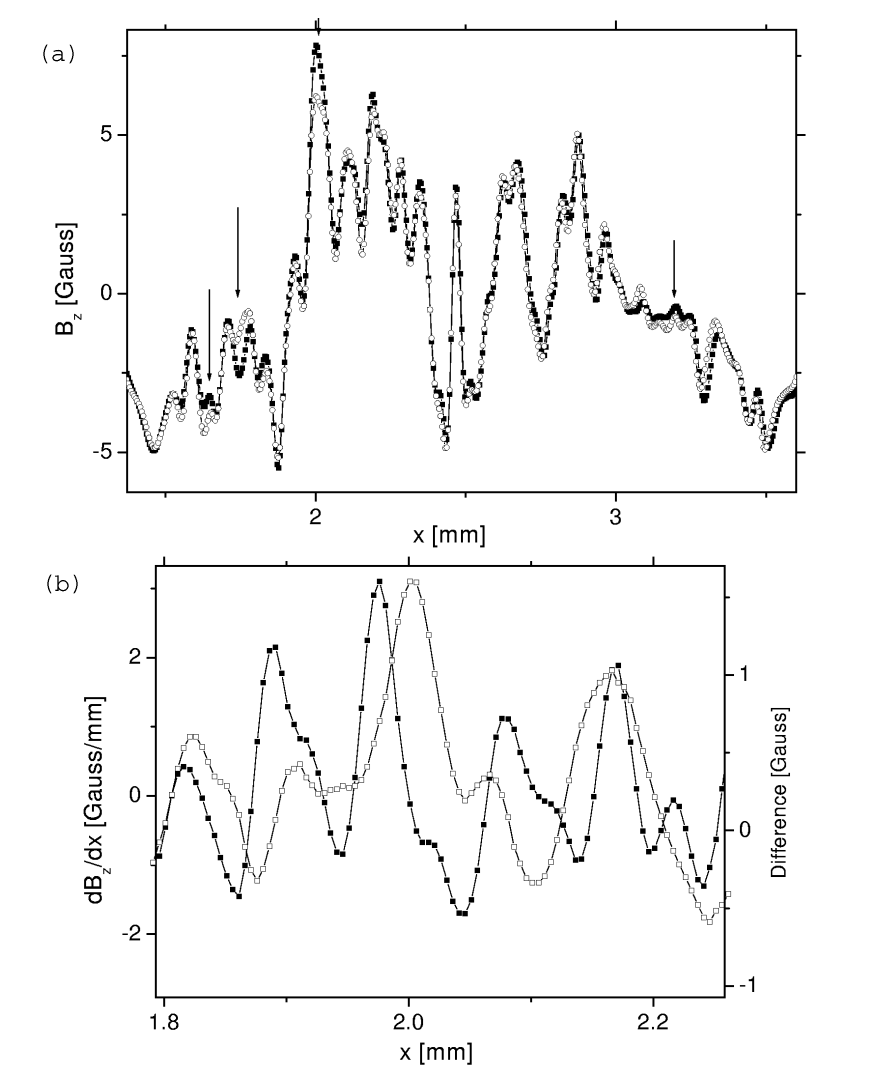
\includegraphics[width=5.7in]{figs/magpen/dclineclose.ps}
\caption[Before and after line cuts of DC hysteresis 
images at a height of $15\,\micron$.]
{(a) 
Vertical line cuts of DC hysteresis images, with the SQUID at a height of
$15\,\micron$, at $x=7.5\,\mm$. 
Zero field cooled line scan (open circles) and line scan after 
ramping the external field to $1.16\,\Oe$ and back to zero
(black squares). 
(b) Difference (black squares) and gradient (open squares) of the
vertical line cuts.
}
\label{fig:dc_hist_cuts_low_a}
\label{fig:dc_hist_cuts_low_b}
\end{figure}


%
% fig8 - DC hyst at 15 microns
%	part 1 
%
%\begin{figure}
%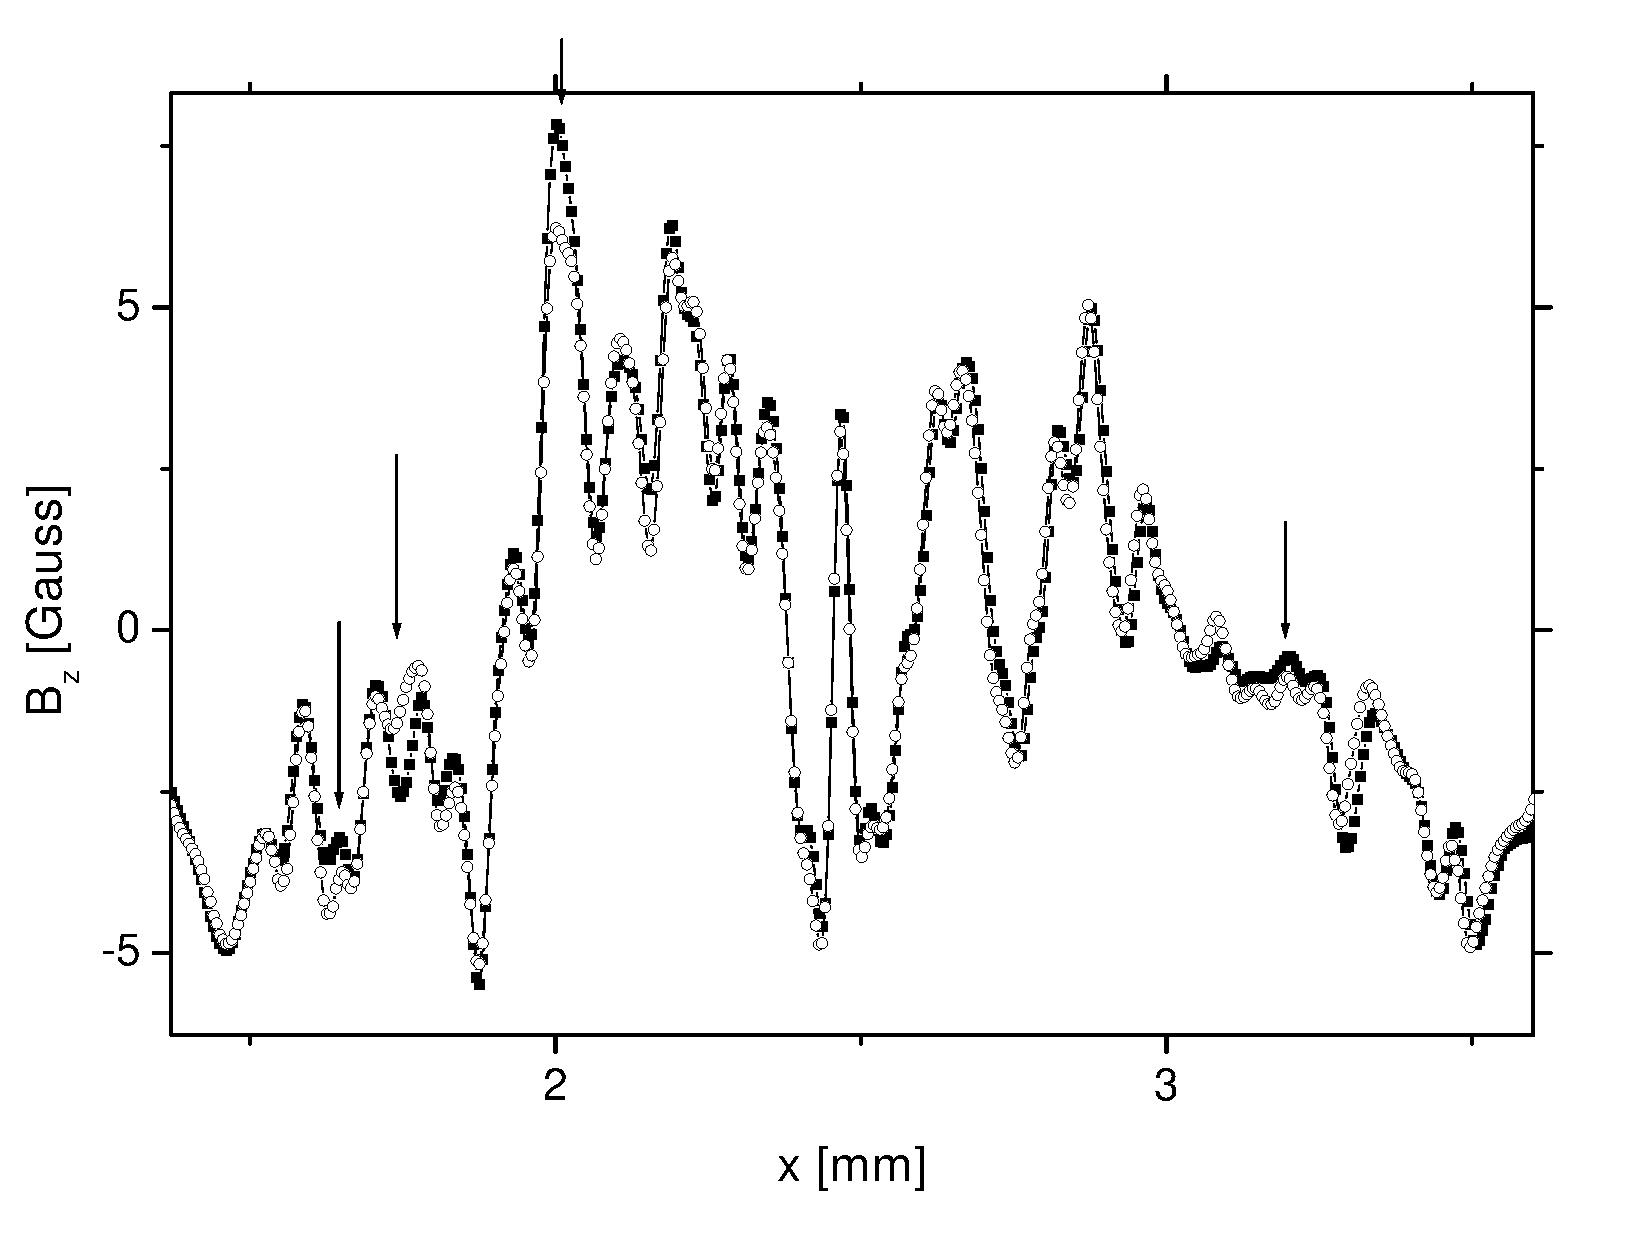
\includegraphics[width=5.7in]{figs/magpen/fig8a.eps}
%\caption[Before and after 
%DC hysteresis line scans at a SQUID height of $15\,\micron$.]
%{Before and after
%DC hysteresis line scans at a SQUID height of $15\,\micron$. These line
%scans are taken at the same location at those in 
%\FigRef{fig:dc_hist_cuts_high_a}, $x=7.5\,\mm$. 
%Zero field cooled line scan (dark squares) and line scan 
%after ramping external field to $1.16\,\Oe$ and back to zero
%(open circles).
% }
%\label{fig:dc_hist_cuts_low_a}
%\end{figure}

%
% fig8 - DC hyst at 15 microns
% 	part 2
%
%\begin{figure}
%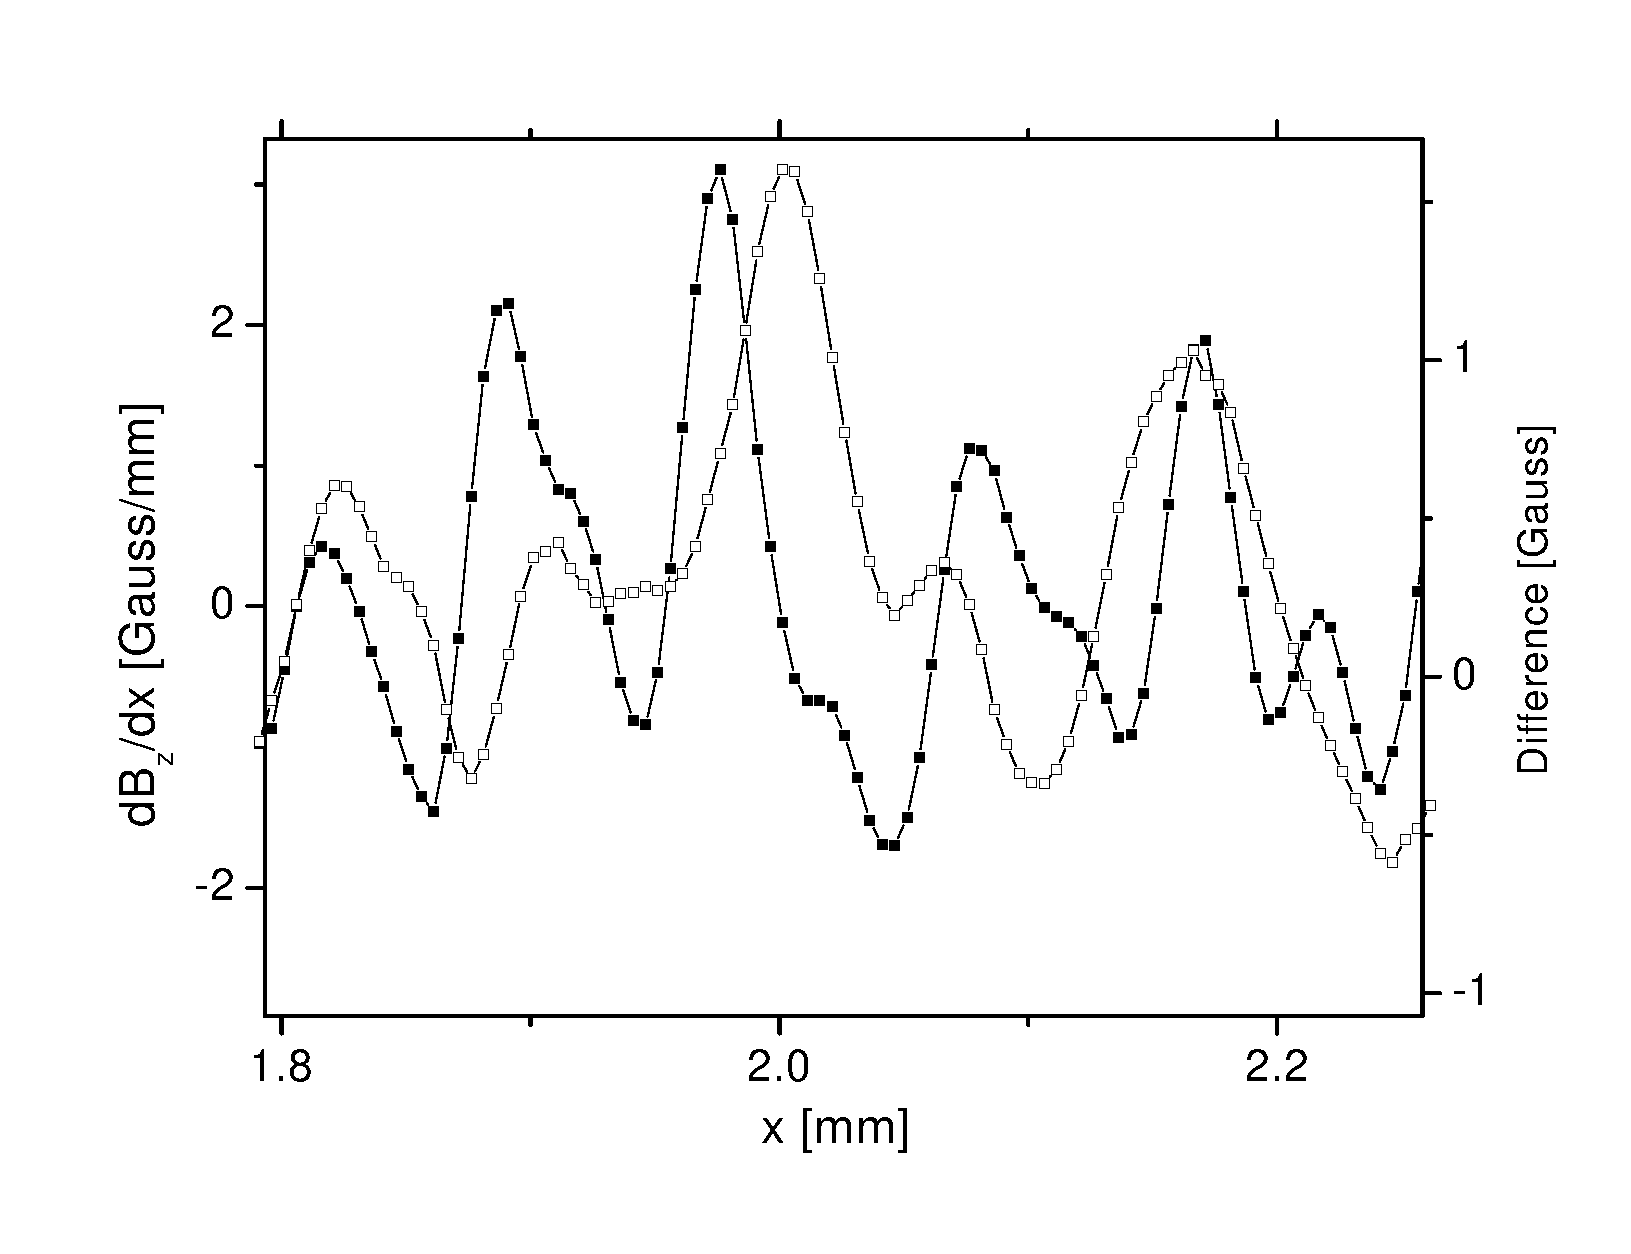
\includegraphics[width=5.7in]{figs/magpen/fig8b.eps}
%\caption[Difference and gradient 
%DC hysteresis line scans at a SQUID height of $15\,\micron$.]
%{Difference and gradient
%DC hysteresis line scans at a SQUID height of $15\,\micron$. These line
%scans are taken at the same location at those in 
%\FigRef{fig:dc_hist_cuts_high_a}, $x=7.5\,\mm$. 
%Difference of the two line scans in \FigRef{fig:dc_hist_cuts_low_a}
%(dark squares)
%and the gradient of the zero field cooled line scan (open
%squares). This image is zoomed in to part of the total range
%to enhance clarity between peaks.
%The solid lines are a guide for the eye for both figures.
% }
%\label{fig:dc_hist_cuts_low_b}
%\end{figure}

%
% some sort of RABITS conclusion
%
The comparison of \FigRef{fig:dc_hist_cuts_high_a} and 
\FigRef{fig:dc_hist_cuts_low_a} is quite revealing. With the SQUID
at a height of $50\,\micron$ there is very little structure in the
line scans. The line scans at a height of $15\,\micron$ have a 
very peaked structure, demonstrating that flux is becoming trapped
in the sample. In fact, we can compare the distance between the peaks,
to the average distance between the holes (\cf\ \FigRef{fig:optical_rabits})
which the YBCO/RABiTS sample presents. 

\section{Magnetic penetration into YBCO thin films}
\label{sec:magpen_ybco}

\subsection{Experimental details}
\label{sec:magpen_exp_details}
%
% experimental details
%
Because several authors (\cf\ Zeldov\etal\,\cite{zeldov_prl_73_1428_1994}
and Kuznetsov \etal\,\cite{kuznetsov_prb_59_1507_1999}) predict
remanence to occur in different ways (center versus edge pinning
of vortices),
we studied thin superconducting $\ybco$ films
in an external field applied perpendicular to the
plane of the sample using a scanning SQUID microscope 
(SSM) \cite{black_apl_62_2128_1993}.
Furthermore, we know of no experimental measurements of
the field nor current distributions in the Meissner state for
a film, such as ours, with a large demagnetizing factor. Because
we use a SQUID we are able to make sensitive low-field measurements which
other techniques (such as magneto optical indicator films or 
scanning Hall
probes) cannot provide. 

The films were deposited using pulsed laser deposition onto a strontium 
titanate
substrate, in a process similar
to that used for depositing YBCO onto nickel based RABiTS tapes
\cite{feldman_apl_77_2000,feldman_2000,rabits_web}.
The films had a size of  $1\,\micron \times 3\,\mathrm{mm}
\times 15\,\mathrm{mm}$.
This particular sample had a wire patterned into the center
(\cf\ \MultFigRef{fig:optical_rabits}{b}).
Because of experimental probe design limitations, 
we could thermal cycle samples above $100\,\kelvin$, but could not 
make any measurements near the transition temperature.
The measurements described here are all at $4.2\,\kelvin$. 


\subsection{Meissner state}
\index{Meissner state|(emph}
\label{sec:ybco_meissner_state}

%
% Meissner state discussion
%
We first studied the sample in the Meissner state. To verify that the 
sample remained in the Meissner state we zero field cooled
the sample, ramped the external field from zero to a specific value
and then ramped the external field back to zero. By comparing the
image after zero field cooling with the image after ramping the
external field up and down, we determined if any flux became trapped
in the sample. If no flux became trapped in the sample
the sample was assumed to be in the Meissner state up to the specified value
of external field.\footnote{It is possible, but very unlikely, that flux
entered and left the sample reversibly, see the discussion on
p.~\pageref{sec:flux_motion_losses}. }
We found that our sample remained in the Meissner state for external 
fields less than $223\,\mOe$ but became hysteretic for fields greater than 
$448\,\mOe$. Fig.~\ref{fig:meissner_image}
shows  the sample in the 
Meissner state at $223\,\mOe$. 

%
% fig9 - Meissner State Image
%        equivalent to fig 3 in magpen paper
%
\begin{figure}[p]
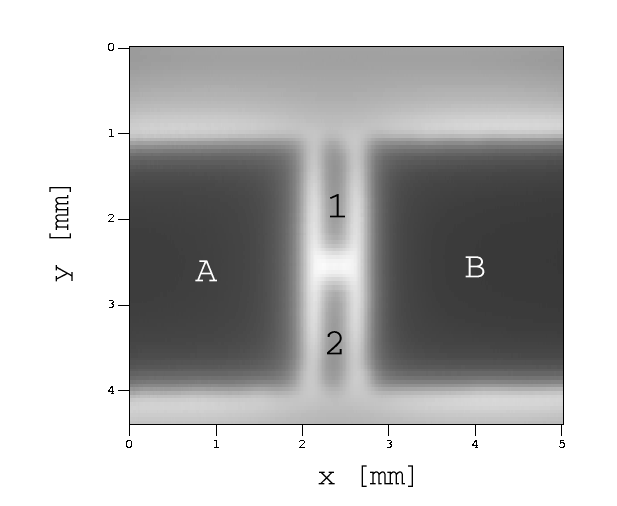
\includegraphics[width=5.7in]{figs/magpen/fig9.ps}
\caption[Meissner state image and line cut of YBCO film on STO.]
{Magnetic image of the YBCO film in a $223\,\mOe$
applied field. The grey scale indicates average magnetic field in the 
SQUID  ranging from 
zero (black) to $1.2\,\Gauss$ (white). The superconductor is 
in the black colored regions, where it is screening flux, labeled A and B.
The 
superconductor is $3\,\mm$ wide. In the center of the superconductor
a wire (not visible) 
for transport measurements is patterened, leaving two 
sacrificial islands of YBCO, labeled 1 and 2. }
\label{fig:meissner_image}
\end{figure}

Additionally, we verified that the
sample contained no remanence in this case by subtracting the
zero field cooled image from an image taken after increasing
the external field and removing it again. 
Fig.~\ref{fig:remanence_a} shows the results
of this experiment, in which it can be clearly seen that there
is no remaining flux pinned in the sample. We note there are some 
changes, notably the circular regions in the center. These circular
regions are damaged regions where contact pads where pushed 
into the sample for testing of transport parameters, and should not
be considered representative of the typical sample properties. 
The grey scale in Fig.~\ref{fig:remanence_a}  
goes from $-1.3\,\mGauss$ to $1.3\,\mGauss$
which corresponds to 
the flux sensitivity resolution
level in our experiment of $\pm 1.3 \,\mGauss$ for
measurements (such as the remanence measurements presented here)
which require the addition or subtraction of two images. 
Contributions to the noise level include flux noise in the
SQUID, and displacement errors in the scanning process.

%
% fig 11 - Remanence measurement comparisons
%	part 1
%
\begin{figure}[p]
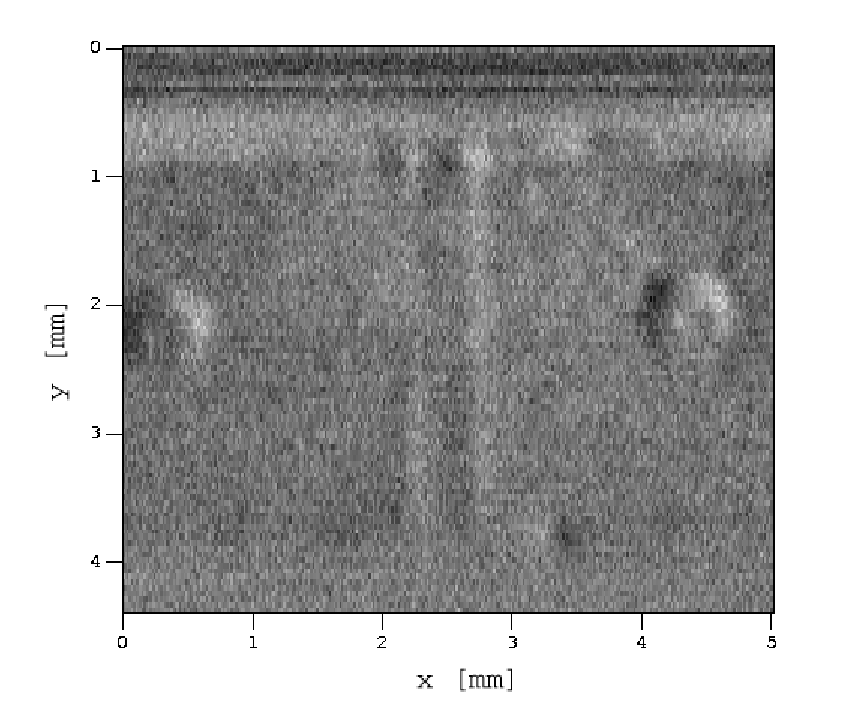
\includegraphics[width=5.7in]{figs/magpen/fig11a.eps}
\caption[Remanence image of YBCO/STO film after peak field of
$223\,\mOe$.]
{Remanence image of the YBCO film after cooling in zero
field and then ramping the external field to 
$223.\,\mOe$.
The grey scale runs from $-1.3\,\mGauss$ (black) to $1.3\,\mGauss$ (white).
 }
\label{fig:remanence_a}
\end{figure}

The flux difference measured in \FigRef{fig:remanence_a} 
is three orders of magnitude smaller than the flux difference measured in 
Fig.~\ref{fig:remanence_b} or 
\FigRef{fig:meissner_image}. The latter two flux difference levels 
are representative
of the flux difference levels measured throughout the course of this
experiment, \ie\ the in-field Meissner state discussion to follow. 

We have additionally made a line cut through the image shown in
Fig.~\ref{fig:meissner_image} at $y=3.5\,\mathrm{mm}$. 
The data points for this line cut are shown in 
Fig.~\ref{fig:vodo_comparison}. The 
current distribution which generates this magnetic field profile
can be inferred by comparing with the data. Because our sample is
so long compared to the width ($15\,\mathrm{mm}$ \vs\ $3\,\mathrm{mm}$)
we treat it as an infinitely long superconductor of width 
$2 W=3\,\mathrm{mm}$ and thickness $d = 1\,\micron$.
Additionally, 
we define the thin film penetration depth
$\lambda_\perp = 2 \lambda^2/d$ where $\lambda$ is the
\index{London penetration depth}% 
London penetration depth and $\lambda_\perp$ is the thin film
penetration depth, as discussed in Pearl \cite{pearl_lt9_566_1965,%
pearl_apl_5_65_1964}.

\index{London equation}%
Starting from the London equation and Ampere's law, we can derive
an integrodifferential equation describing the current distribution
in a thin film. This derivation is non-trivial, but a careful 
analysis has been carried out by Dorsey \cite{dorsey_prb_51_15329_1995}.
This integrodifferential equation is
%
\begin{equation}
{\lambda_\perp \over 2} {\partial I(x) \over \partial x} = 
{1 \over 2 \pi} \int_{-W}^{W} {I(x') \dif x' \over x'-x} - H_{\mathrm{ext}}
\label{eqn:intdifeqn}
\end{equation}
%
in which $I(x) = \int J(x,z)\,\dif z$, the two-dimensional 
current density.

There is a well known solution to \EqnRef{eqn:intdifeqn} due to 
Larkin and Ovchinikov \cite{larkin_jetp_34_651_1972} for the 
current distribution interior to the sample. 
If $\lambda_\perp \ll W$ we neglect the left hand side of 
\EqnRef{eqn:intdifeqn} and solve to get
%
\begin{equation}
I(x) = - { 2 H_\mathrm{ext} x \over \sqrt{W^2 - x^2}}, 
\label{eqn:LO_result}
\end{equation}
%
with $x$ as the 
coordinate along the width of the film.
This diverges at the sample edge, so cannot be valid everywhere. 
\EqnRef{eqn:LO_result}\ does not contain any dependence 
upon the penetration depth since we neglected that term in 
\EqnRef{eqn:intdifeqn} to form the solution. 

Larkin and Ovchinikov also found a form for the current
distribution at the sample edge, valid only in the edge region, 
but did not discuss the cross over region.%
\footnote{There is an error in the Larkin and Ovchinikov edge formulation,
noted by Dorsey \cite{dorsey_prb_51_15329_1995}. In both cases,
the maximum value of the current
(\cf\ Eqn.~\ref{eqn:current_maximum}), at the edge, is however,
given correctly, and agrees with the asymptotic results given
by Vodolazov and Maksimov\cite{vodolazov_physc_349_125_2001}.
}




%
% fig 10 - Meissner state experiment comparison with Vodolazov et al.
%          equivalent to figure 4 in magpen paper
%
\begin{figure}[p]
\includegraphics[width=5.7in]{figs/magpen/fig10.ps}
\caption[Comparison of Meissner state field profile with 
Vodolazov \etal\ predictions.]
{Comparison of line cut (black dots) in 
Fig.~\ref{fig:meissner_image}
with the magnetic field predictions for $-2\,\mm<x<2\,\mm$ 
of Vodolazov \etal\ (solid line).
We used the following parameters to generate the specific curve, with 
the caveats noted in the text: $\lambda = 150\,\nm$, 
$H_{\mathrm{ext}}=200\,\mOe$, a SQUID height of $175\,\micron$
and the sample's geometric parameters.  
}
\label{fig:vodo_comparison}
\end{figure}


Instead, we chose to look at the
Vodolazov and Maksimov\cite{vodolazov_physc_349_125_2001} results:
an asymptotic form for the current 
distribution in the sample, for the case of a thin film $d<\lambda$ and
a thick film $\lambda < d < W$, valid over the entire cross section
of the sample.  They find that 
the results in both the thin and thick
cases closely agree, except near the edge region
$\left| x \right| < W - d$, and that both solutions agree for the 
maximum value at
$\left| x \right| = W$. 
They predict this edge value, which is the maximum value of the current 
distribution, 
%
\begin{equation}
{I(W)\over H_{\mathrm{ext}}}= \sqrt{2\pi{ W \over \lambda_\perp }}.
\label{eqn:current_maximum}
\end{equation}
%

We compared our measured magnetic field profile with the 
profile predicted by Vodolazov
and Maksimov
%
\begin{equation}
I(x)=H_{\mathrm{ext}} {x \over \sqrt{\alpha (W^2-x^2)+\beta}},
\end{equation}
%
with $\alpha = \frac{1}{4} - \frac{0.63}{(W/\lambda_\perp)^{0.5}} 
+ \frac{1.2}{(W/\lambda_\perp)^{0.8}}$ and 
$\beta = \frac{2 \lambda_\perp}{\pi W} + 4(\frac{\lambda_\perp}{W})^2$. 
With this model we found the best comparison to occur for 
a SQUID height of $175\,\micron$
and an external field of $200\,\mOe$. These values compare 
favorably to the experimental parameters: an estimated 
SQUID height of $100\,\micron$ and an external
field of $223\,\mOe$.  
Additionally we find that we can compare the data with any value of 
$\lambda$ of about $1\,\micron$ or less; this occurs because
our resolution is limited by the height of the SQUID over the sample.
Consequently, we cannot extract a value for $\lambda$ from our
data. However, there is quite good agreement between the data and
the model using our parameters, as shown in \FigRef{fig:vodo_comparison}.

\index{Meissner state|)}%
  

\subsection{Demagnetization factor}
\index{demagnetization factor}%
\index{\hcone|(emph}%

%
% Demag factor and H_c1
%
We computed the demagnetization factor for the sample we used
by comparing the value of the applied external field  compared
to the measured magnetic field near the edge of the sample, using 
%
\begin{equation}
\eta = 1 - {H_{\mathrm{ext}} \over H_{\mathrm{edge}}}
\label{eqn:demag_def}
\end{equation}
%
in which $H_{\mathrm{ext}}$ is the applied external field and
$H_{\mathrm{edge}} $ is the magnetic field as measured at
the edge of the sample. 
%Because we are not at the surface of the sample
%(the SQUID is a distance above) we are able to provide only a lower bound
%on $\eta$. We only consider measurements made in the Meissner state
%because once flux penetrates the sample $H_{\mathrm{edge}}$ decreases
%and will change the result. We find a lower bound for the 
%demagnetization factor for our
%sample to be $\eta = 0.552$. 
We take the model parameters, generated above,
and use them, by setting the SQUID height to zero, to compute
the magnetic field at the edge of the sample, $H_{\mathrm{edge}}=5770\,\mOe$.
This value of $H_{\mathrm{edge}}$ yields a demagnetization factor of 
$\eta = 0.961$. 

Once we know the demagnetization factor we can provide an estimate of
$H_{c1}$, the first critical field of the sample. 
When $H_{\mathrm{edge}}$ exceeds 
$H_{c1}$, flux begins to penetrate the sample in the form 
of vortices. Because of observed flux pinning in the sample, flux does 
not penetrate further into the sample, and also remains
pinned even when the external field is removed. From the
observation of first flux penetration we obtain a measurement
of $H_{c1}$.
We used our values for the demagnetization factor at the surface
of the sample to estimate $H_{c1}$ for this film to be between
$5.77\,\Oe$ (for which the sample remains in the Meissner state) 
and $11.48\,\Oe$ (for which we first notice flux penetration).
We can compare this range to what one would expect for bulk samples. 
From Tinkham\footnote{Tinkham\,\cite{tinkham}, p.~149.}
the first critical field is defined as the external magnetic field
at which the free energy becomes metastable with respect to the formation
of the first vortex. The value of this critical field in the bulk
is
%
\begin{equation}
H_{c1} = {1 \over 4\pi} {\Phinot \over \lambda^2} \ln\kappa\mbox{,}
\end{equation}
%
in which $\kappa=\lambda/\xi$ the ratio of the London penetration
depth to the superconducting coherence length. 
Using $\lambda = 2000\,\angstrom$ and $\xi= 1 \,\nm$ we find a bulk 
value of $H_{c1} = 220\,\Gauss$. 

By contrast, Kuznetsov\cite{kuznetsov_prb_59_1507_1999} provides a 
form for \hcone\ in the case of a thin film ($d < \lambda$),
%
\begin{equation}
H_{c1f} \approx {\Phinot \over 16 (2 \ln 2 +1) \lambda_\perp W}
    \left( \ln{\lambda_\perp\over r_c} + 0.81 \right)\mbox{,}
\label{eqn:kuzn_hc1}
\end{equation}
%
in which $r_c$ is the radius of the vortex core and is taken to be
$r_c \approx \xi$. \EqnRef{eqn:kuzn_hc1}\ already accounts for the 
demagnetizing factor, so 
the Kuznetsov formula 
gives a value of $H_{c1} = 250 \,\mGauss$, which is considerably smaller
than the bulk value, but is in excellent agreement with our applied field
of $223\,\mOe$.

The inferred value of $H_{c1}$ from the flux penetration measurements,
in the case of the bulk value, is too small. However, in the thin film case
the value of \hcone\ agrees quite nicely between our experiment and
Kuznetsov \etal\cite{kuznetsov_prb_59_1507_1999} This indicates that
our sample can be well described by the thin film limit ($d<\lambda$) 
despite the fact that our sample is actually slightly \emph{thicker}
($d=1\,\micron$)
than the penetration depth ($\lambda\approx 2000\,\angstrom$).

\index{\hcone|)}

\subsection{Remanence in YBCO films}
\index{remanence}
\index{critical state}
%
% remanence discussion
%
In addition to the Meissner state, we looked at the 
critical state, for external fields up to $57.4\,\Oe$. 
Fig.~\ref{fig:remanence_b}\ shows the remanence after zero
field cooling the sample, applying a $57.4\,\Oe$ external
field to it, and then removing the sample. The flux became
trapped near the edges of the sample. This picture differs
quite dramatically from that of the geometrical barrier
\cite{zeldov_prl_73_1428_1994} 
and even from the description of vortex penetration given
by Vodolazov and Maksimov for thick films
\cite{vodolazov_physc_349_125_2001},
in which remnant flux becomes
trapped in the \emph{center} of the sample. 

Kuznetsov \etal\,\cite{kuznetsov_prb_59_1507_1999} give a
different picture of flux penetration and the critical
state flux distribution in which flux penetrates the sample 
and, because of strong pinning sites, becomes
pinned at the edge region and does not penetrate into the 
center of the sample. In fact the Kuznetsov \etal\ picture
looks remarkably similar to the flux distribution seen 
in our experiment.

%
% fig 11 - Remanence measurement comparisons
%	part 2
%
\begin{figure}[p]
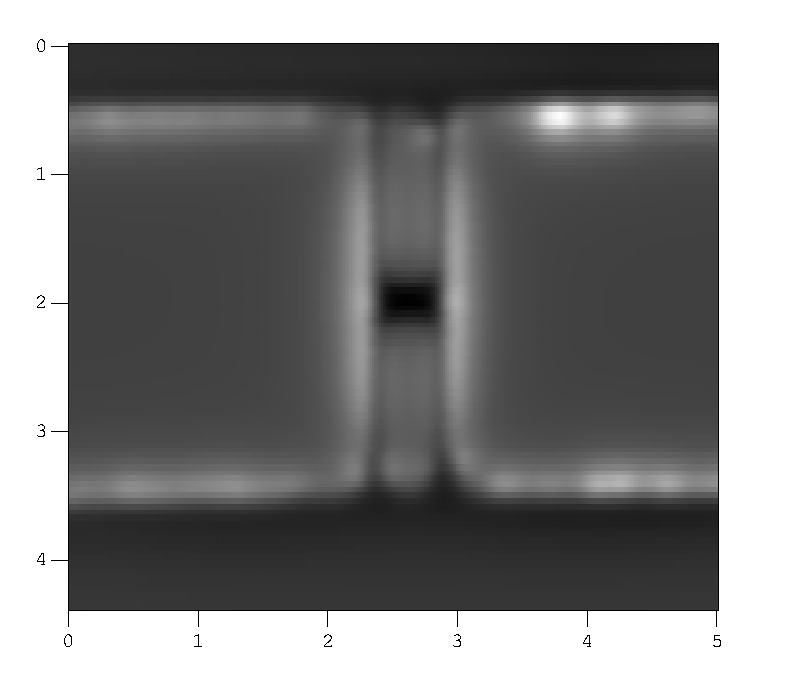
\includegraphics[width=5.7in]{figs/magpen/fig11b.eps}
\caption[Remanence image of YBCO/STO film after peak field of
$57.4\,\Oe$.]
{Remanence images of the YBCO film after cooling in zero
field and then ramping the external field to 
$57.4\,\Oe$ and back to zero. The grey scale runs from $-1.3\,\Gauss$ (black)
to $2.15\,\Gauss$ (white). 
 }
\label{fig:remanence_b}
\end{figure}

Kuznetsov \etal\ give specific analytic predictions for the 
current distribution in the critical state.
However, the size of the critical region relates to the magnitude
of the external field. We cannot generate a large enough magnetic
field in the scanning SQUID microscope to create a large enough
critical region to analyze. This occurs because our resolution is
limited
by the SQUID-sample separation and we cannot resolve features
of the size needed to quantitatively 
compare with the Kuznetsov \etal\
model. 

We can observe that the size of the critical region grows as the
externally applied field is increased. \FigRef{fig:remanence_line_cuts}
shows the magnetic field profile for the sample as the external field
increases from $0\,\Oe$ to $44.9\,\Oe$ to $57.4\,\Oe$. 

%
% fig 12 - remanence line cuts
%          equivalent to fig 5 in magpen paper
%
\begin{figure}[p]
\includegraphics[width=5.7in]{figs/magpen/fig12.eps}
\caption[Magnetic field profiles of the remanence critical state in 
YBCO films.]{Magnetic field profiles on the remanence critical state in 
the YBCO/STO film.  for $H_{\mathrm{ext}}= 57.0\,\Oe$ (black squares) 
$44.9\,\Oe$ (open circles) and $11.2\,\Oe$ (open triangles) 
}
\label{fig:remanence_line_cuts}
\end{figure}

%
% conclusions 
%
To conclude, we have imaged both the Meissner state and the critical state in
a YBCO film of large demagnetizing factor. From these image 
measurements, we have provided a direct estimate for $H_{c1f}$ in 
YBCO and for the demagnetizing factor for our sample. 
What's more, we have been able to observe the onset of flux penetration
into the sample and to characterize the flux distribution of the 
critical state, finding that flux penetrates the edge of the 
sample and immediately becomes strongly pinned to the edge region
of the sample, in stark contrast to the geometrical barrier picture. 
This edge pinning is due to the strong pinning potential of our
sample, which is quite different from the weak pinning of samples 
such as that measured by Zeldov \etal\,\cite{zeldov_prl_73_1428_1994}
The geometrical barrier is not important in our sample, or in other
sample with large pinning potentials, especially highly granular
thin film materials. In fact, pinning at the edge may be stronger
due to enhanced material defects at the sample edge. 

% 
% comparison of Hclf with Hc1 bulk
%
\index{\hcone}

The value of $H_{c1f}$ that we report here is different from the value
of \hcone\ typically reported in the bulk material
\cite{liang_prb_50_4212_1994}. 
However, this value is about an order of magnitude larger than that
predicted by Kuznetsov
\etal\ for a thin film. The difference between the Kuznetsov \etal\ and 
bulk values arises due to the non-local nature of electrodynamics
in thin films.
The Pearl formulation of thin film electrodynamics
\cite{pearl_apl_5_65_1964,pearl_lt9_566_1965} (used by Kuznetsov \etal)
requires that the thickness of the film be much less than the penetration
depth (\ie\ $d \ll \lambda$). For the sample in our experiment, we do not
fall into this thin film regime ($d=1\,\micron$ and 
$\lambda \approx 1500\,\angstrom$). Our value for 
$H_{clf}$ falls below  the range of reported  
bulk values for \hcone\,\cite{liang_prb_50_4212_1994}, indicating
that our sample falls into some intermediate regime between the thin film
and bulk limits. Many practical devices are made with films of
superconductor and may fall into this regime, so this intermediate
regime may be of important practical consideration in terms of 
understanding the film response.

% LocalWords:  RABiTS YBCO mega STO ORNL rabits SSM Larkin Ovchinikov Mikitik
% LocalWords:  Vodolazov Maksimov Zeldov Kuznetsov Johansen MOIF Ferdeghini zfc
% LocalWords:  Landau pme ext ac lossy Panofsky eqn intergranular reimage dc
% LocalWords:  hyst
